\section*{Введение}

В данной лабораторной работе изучаются матрицы преобразования пространства, которые широко используются в 3D-графике. Основная цель - познакомиться с различными типами матричных преобразований и их применением для создания трехмерных сцен.

\subsection*{Однородные координаты}

В 3D-графике используется система однородных координат, где точка $(x, y, z)$ представляется как $(x, y, z, w)$, где $w$ - однородная координата. Это позволяет объединить линейные преобразования (вращение, масштабирование) и аффинные преобразования (перемещение) в единую матричную форму.

Преобразование из однородных координат в декартовы:
\begin{equation}
(x, y, z) = \left(\frac{x}{w}, \frac{y}{w}, \frac{z}{w}\right)
\end{equation}

\section*{Задание 1: Создание кубика}

\subsection*{Теоретические основы}

Кубик в 3D-пространстве определяется восемью вершинами и шестью гранями. В однородных координатах вершины кубика с ребром длины 2 и центром в начале координат имеют вид:

\begin{equation}
\text{Вершины} = \begin{bmatrix}
-1 & 1 & 1 & -1 & -1 & 1 & 1 & -1 \\
-1 & -1 & 1 & 1 & -1 & -1 & 1 & 1 \\
-1 & -1 & -1 & -1 & 1 & 1 & 1 & 1 \\
1 & 1 & 1 & 1 & 1 & 1 & 1 & 1
\end{bmatrix}
\end{equation}

Грани кубика определяются индексами вершин:
\begin{equation}
\text{Грани} = \begin{bmatrix}
0 & 1 & 5 & 4 \\  % передняя грань
1 & 2 & 6 & 5 \\  % правая грань
2 & 3 & 7 & 6 \\  % задняя грань
3 & 0 & 4 & 7 \\  % левая грань
0 & 1 & 2 & 3 \\  % нижняя грань
4 & 5 & 6 & 7     % верхняя грань
\end{bmatrix}
\end{equation}

\subsection*{Практическая реализация}

Базовый кубик был создан с использованием Python и библиотеки matplotlib. Код включает функции для отрисовки 3D объектов с поддержкой прозрачности и различных цветов.

\begin{figure}[h]
\centering
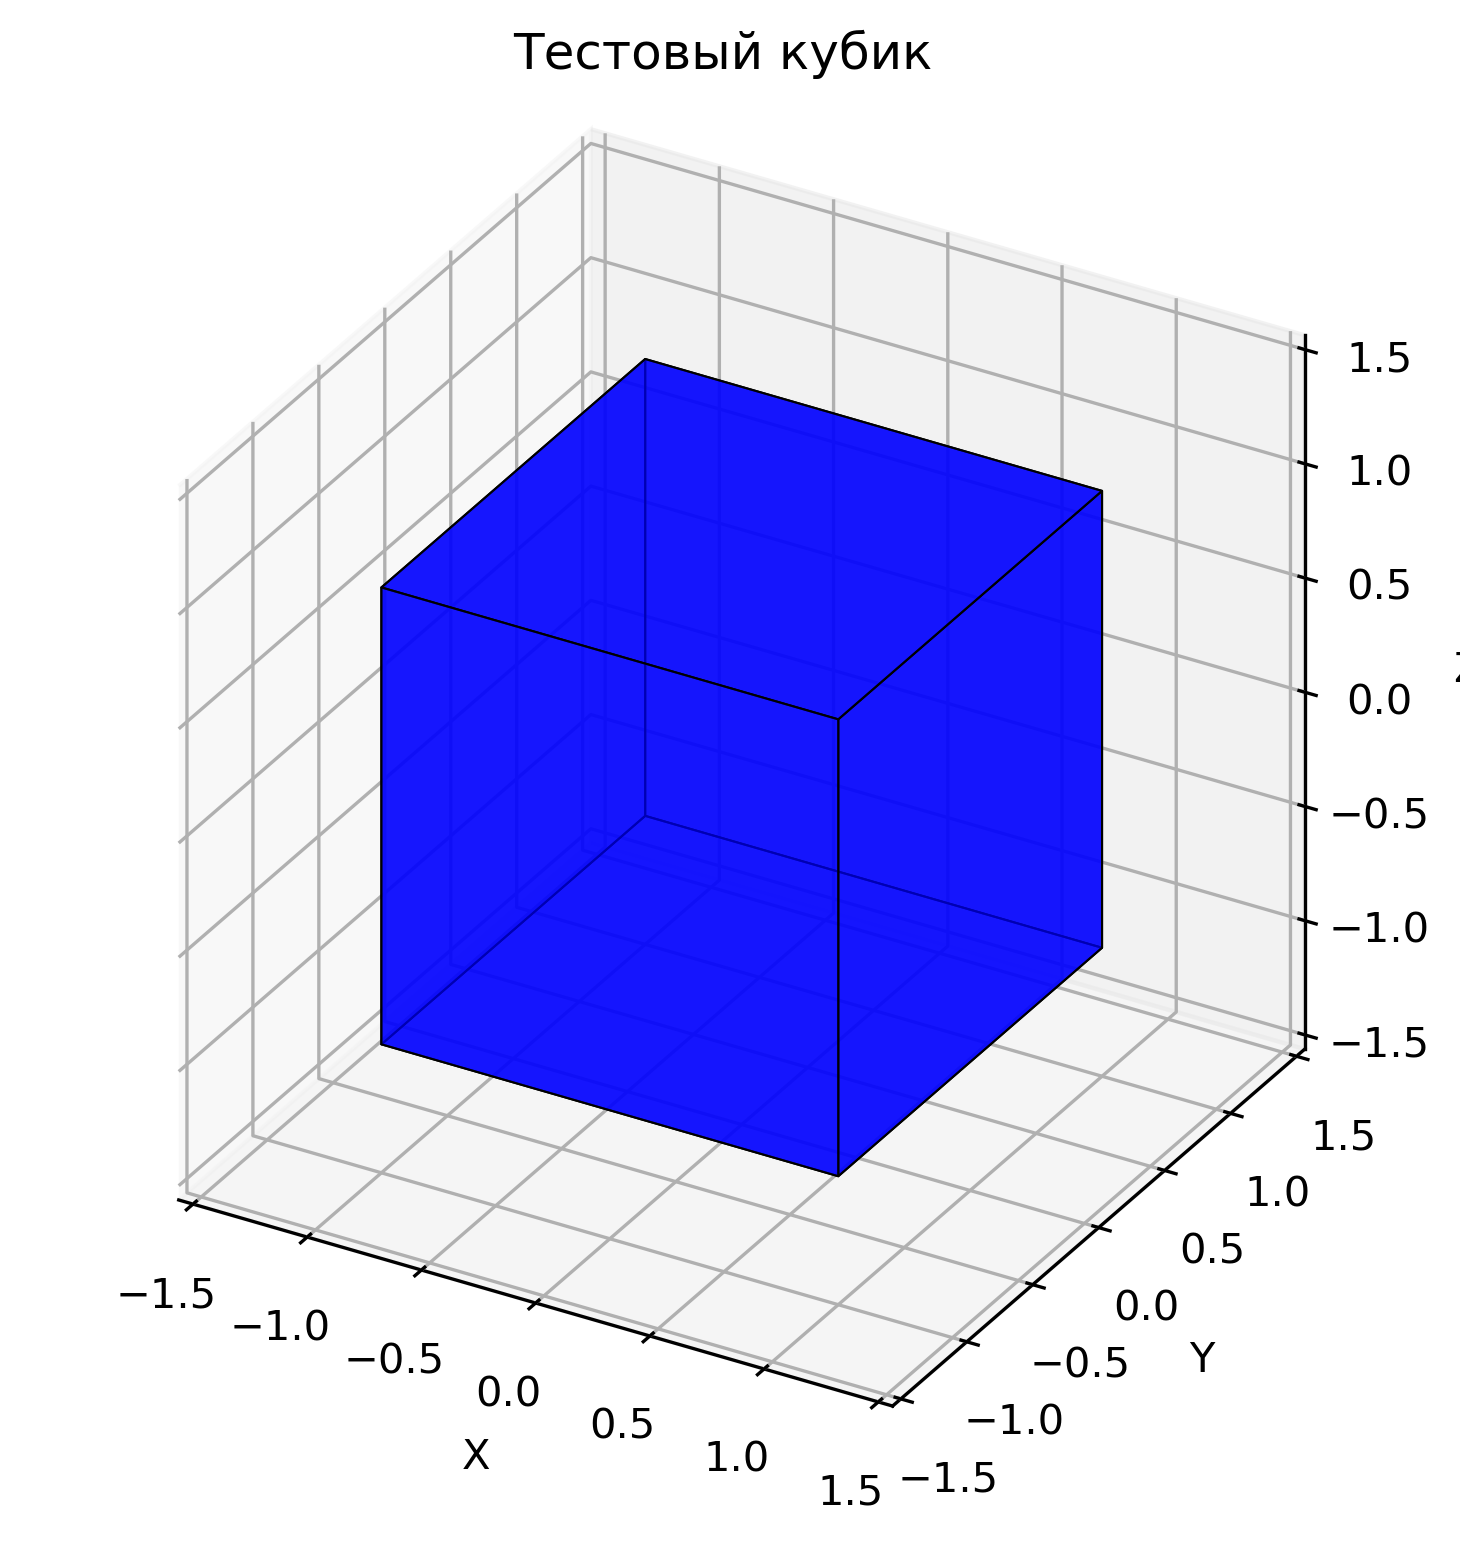
\includegraphics[width=0.6\textwidth]{images/task1/test_cube.png}
\caption{Базовый кубик в 3D пространстве}
\label{fig:basic_cube}
\end{figure}

\subsection*{Почему используются 4-компонентные векторы?}

Использование однородных координат $(x, y, z, w)$ вместо декартовых координат $(x, y, z)$ имеет несколько важных преимуществ:

\begin{enumerate}
\item \textbf{Единообразие преобразований}: Все аффинные преобразования (включая перемещение) можно представить в виде матричного умножения.

\item \textbf{Удобство композиции}: Композиция преобразований сводится к умножению матриц.

\item \textbf{Поддержка перспективы}: Однородные координаты естественным образом поддерживают перспективные преобразования.

\item \textbf{Математическая элегантность}: Все преобразования становятся линейными в однородном пространстве.
\end{enumerate}

\subsection*{Как задать другие фигуры?}

Для создания других 3D фигур необходимо:

\begin{enumerate}
\item \textbf{Определить вершины}: Задать координаты всех вершин фигуры в однородных координатах.

\item \textbf{Определить грани}: Указать индексы вершин, образующих каждую грань.

\item \textbf{Задать цвета и прозрачность}: Для визуализации.

\item \textbf{Использовать функции отрисовки}: Применить те же функции, что и для кубика.
\end{enumerate}

Примеры других фигур:
\begin{itemize}
\item \textbf{Тетраэдр}: 4 вершины, 4 треугольные грани
\item \textbf{Октаэдр}: 6 вершин, 8 треугольных граней  
\item \textbf{Призма}: 6 вершин, 5 граней (2 основания + 3 боковые)
\item \textbf{Пирамида}: 5 вершин, 5 граней (1 основание + 4 боковые)
\end{itemize}

\section*{Задание 2: Масштабирование кубика}

\subsection*{Матрица масштабирования}

Матрица масштабирования $S$ имеет вид:
\begin{equation}
S = \begin{bmatrix}
s_x & 0 & 0 & 0 \\
0 & s_y & 0 & 0 \\
0 & 0 & s_z & 0 \\
0 & 0 & 0 & 1
\end{bmatrix}
\end{equation}

где $s_x$, $s_y$, $s_z$ - коэффициенты масштабирования по осям X, Y, Z соответственно.

\subsection*{Виды масштабирования}

\begin{enumerate}
\item \textbf{Равномерное масштабирование}: $s_x = s_y = s_z = k$
\item \textbf{Неравномерное масштабирование}: $s_x \neq s_y \neq s_z$
\item \textbf{Растяжение по одной оси}: например, $s_x > 1$, $s_y = s_z = 1$
\item \textbf{Сжатие}: $s_i < 1$ для некоторых осей
\end{enumerate}

\begin{figure}[h]
\centering
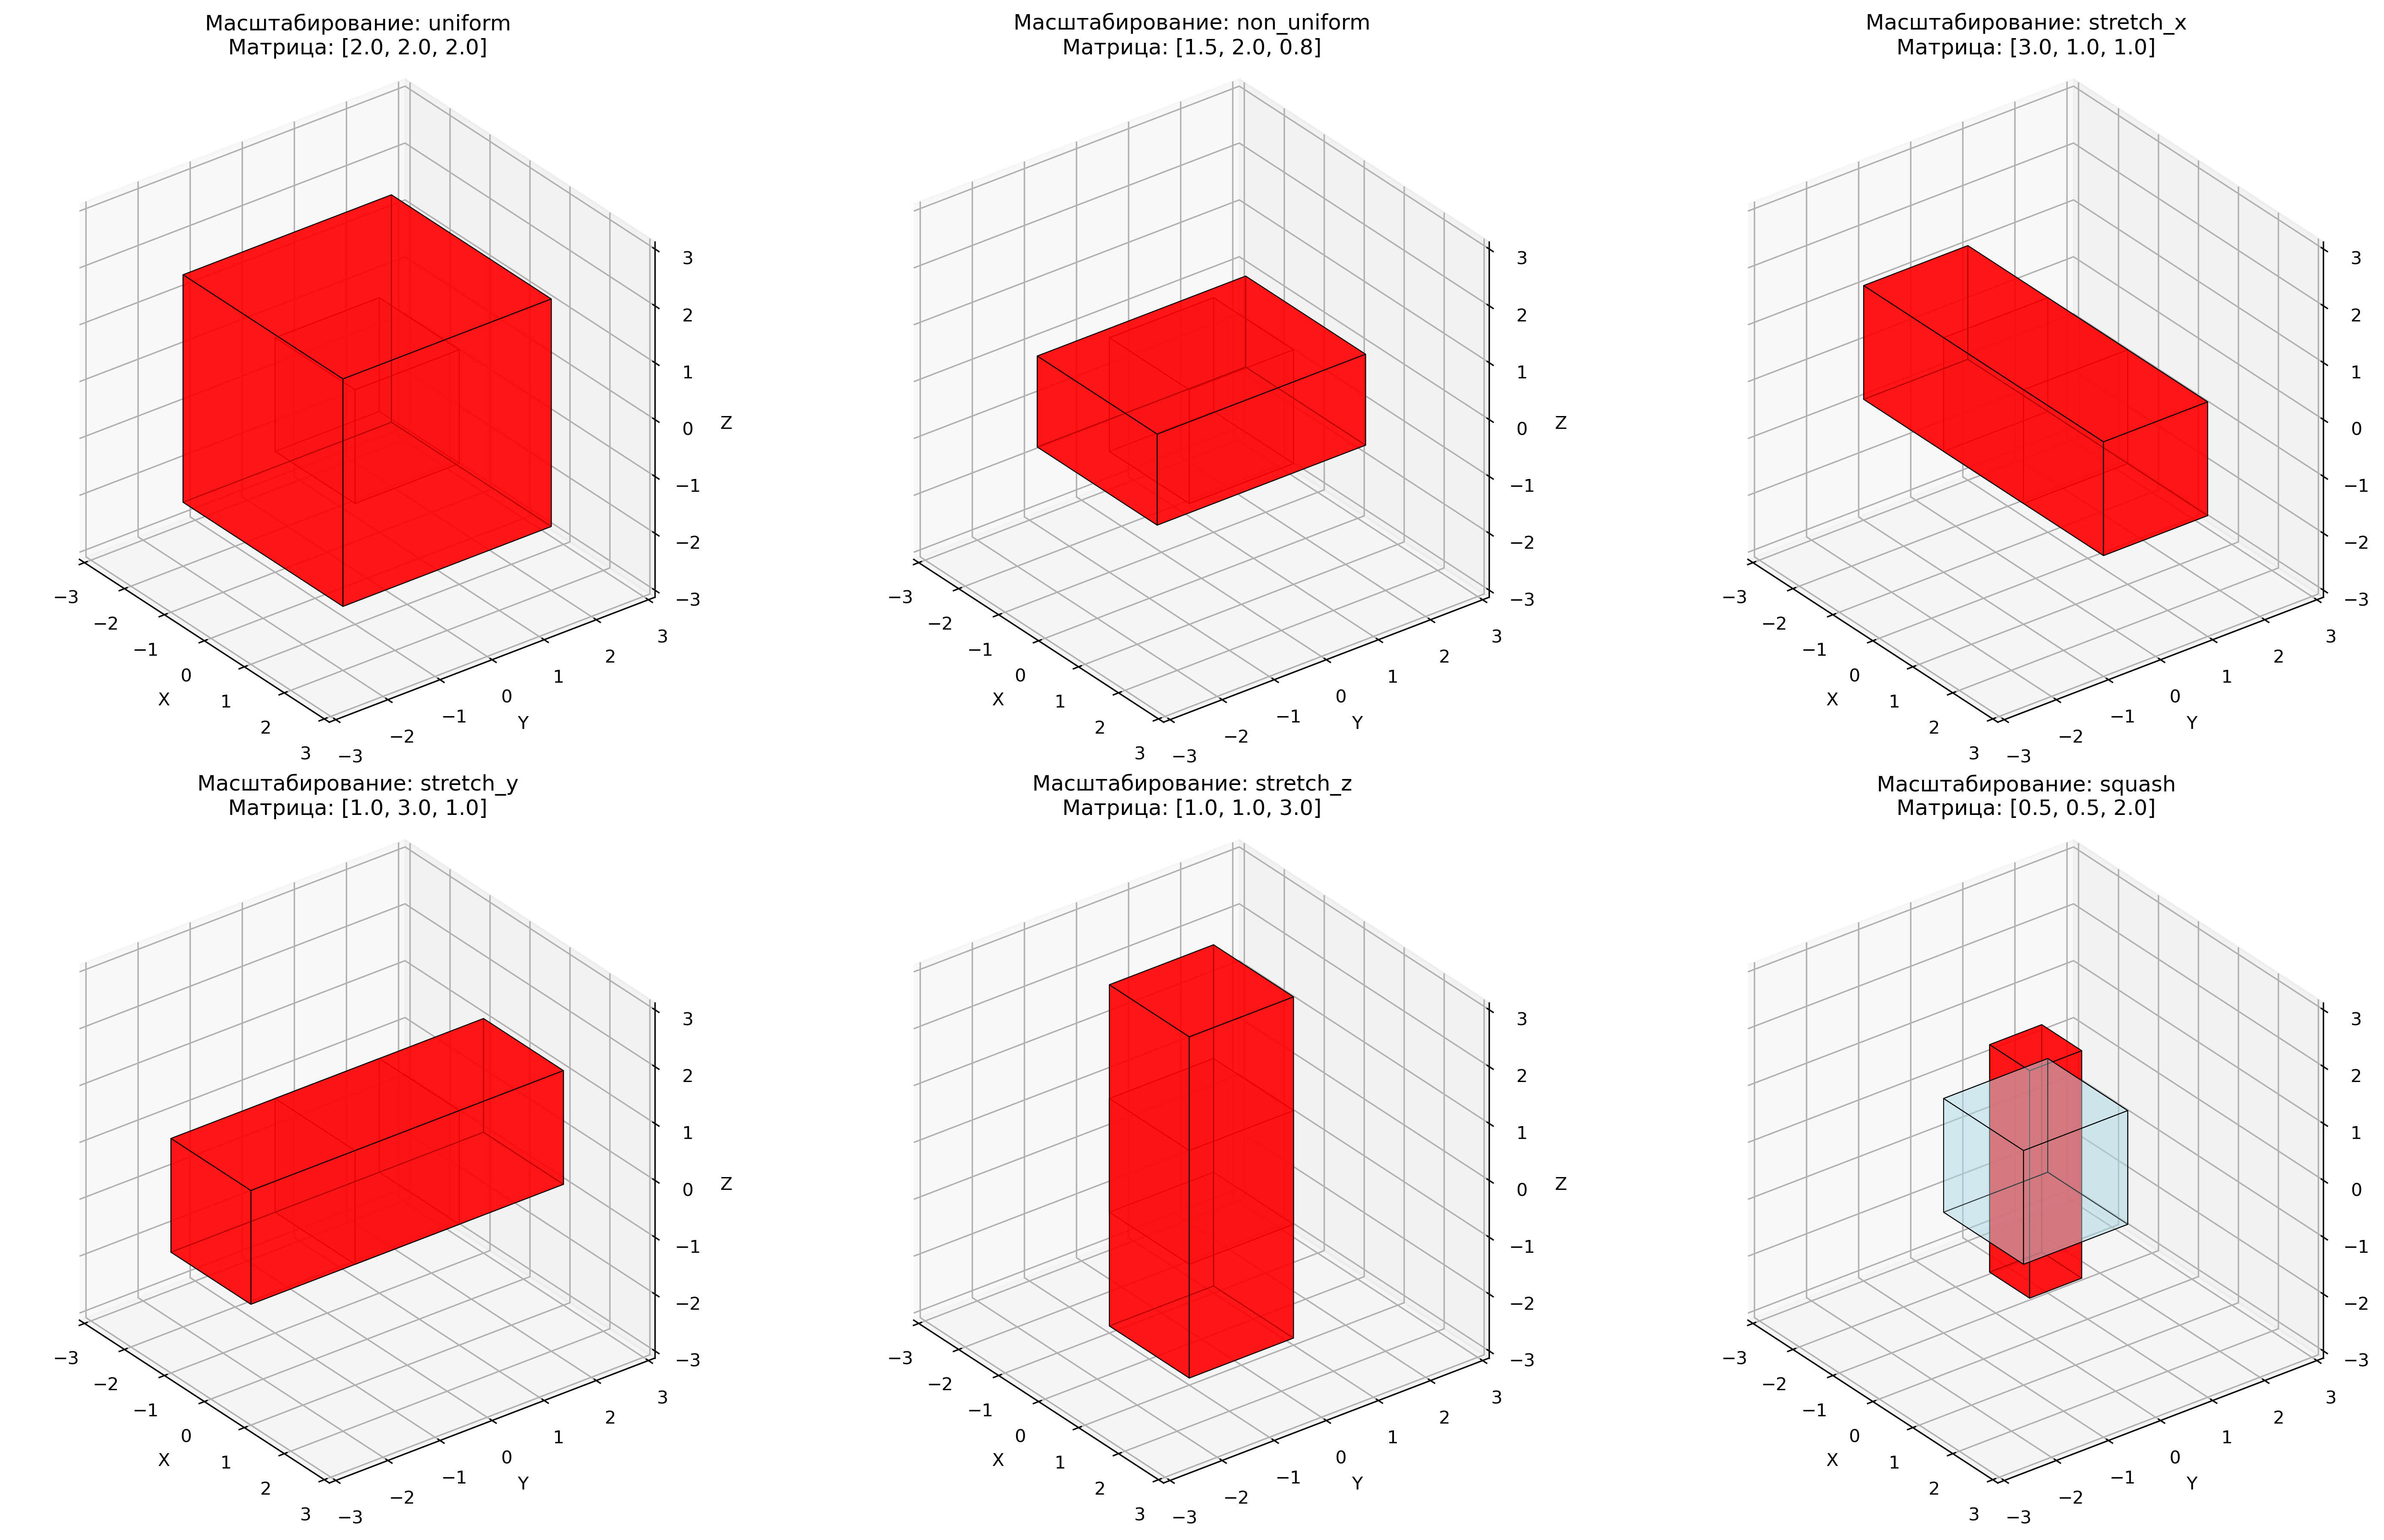
\includegraphics[width=\textwidth]{images/task2/scaling_transformations.png}
\caption{Различные виды масштабирования кубика}
\label{fig:scaling_transformations}
\end{figure}

\subsection*{Сравнение TS и ST}

Важное свойство матричных преобразований - некоммутативность масштабирования и перемещения:

\begin{equation}
TS \neq ST
\end{equation}

где $T$ - матрица перемещения, $S$ - матрица масштабирования.

\begin{figure}[h]
\centering
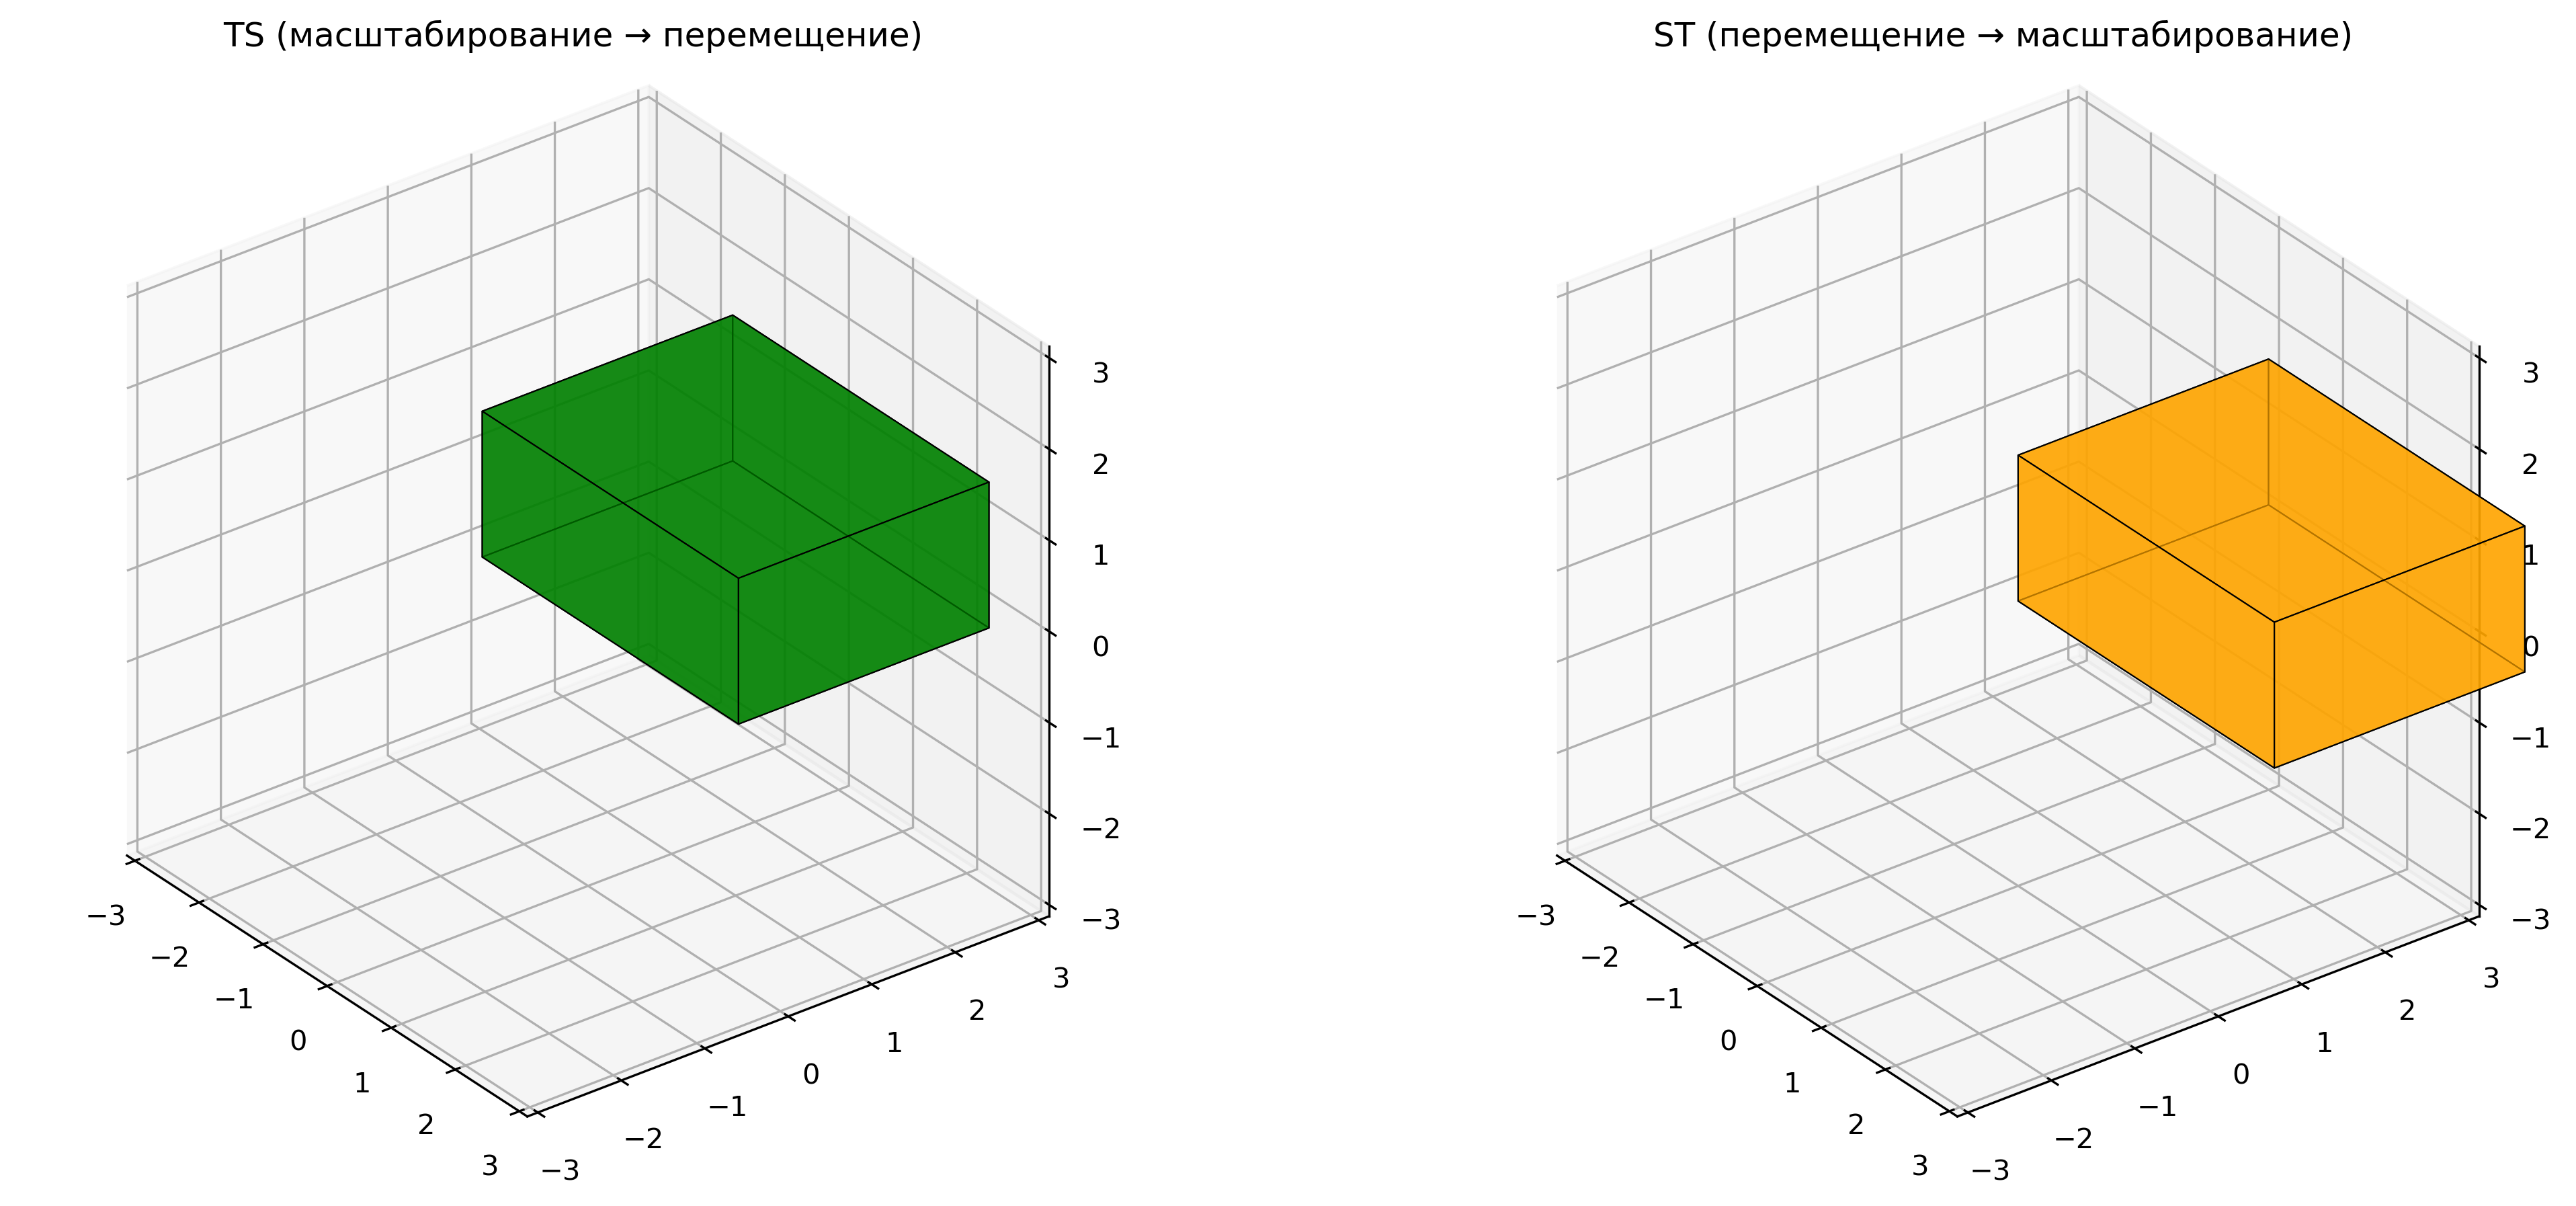
\includegraphics[width=\textwidth]{images/task2/TS_vs_ST_comparison.png}
\caption{Сравнение преобразований TS и ST}
\label{fig:TS_vs_ST_comparison}
\end{figure}

\section*{Задание 3: Перемещение кубика}

\subsection*{Матрица перемещения}

Матрица перемещения $T$ имеет вид:
\begin{equation}
T = \begin{bmatrix}
1 & 0 & 0 & t_x \\
0 & 1 & 0 & t_y \\
0 & 0 & 1 & t_z \\
0 & 0 & 0 & 1
\end{bmatrix}
\end{equation}

где $t_x$, $t_y$, $t_z$ - компоненты вектора перемещения.

\subsection*{Свойства перемещения}

\begin{itemize}
\item Перемещение коммутирует с самим собой: $T_1 T_2 = T_2 T_1$
\item Перемещение не коммутирует с масштабированием: $TS \neq ST$
\item Перемещение не коммутирует с вращением: $TR \neq RT$
\end{itemize}

\subsection*{Демонстрация перемещений}

\begin{figure}[h]
\centering
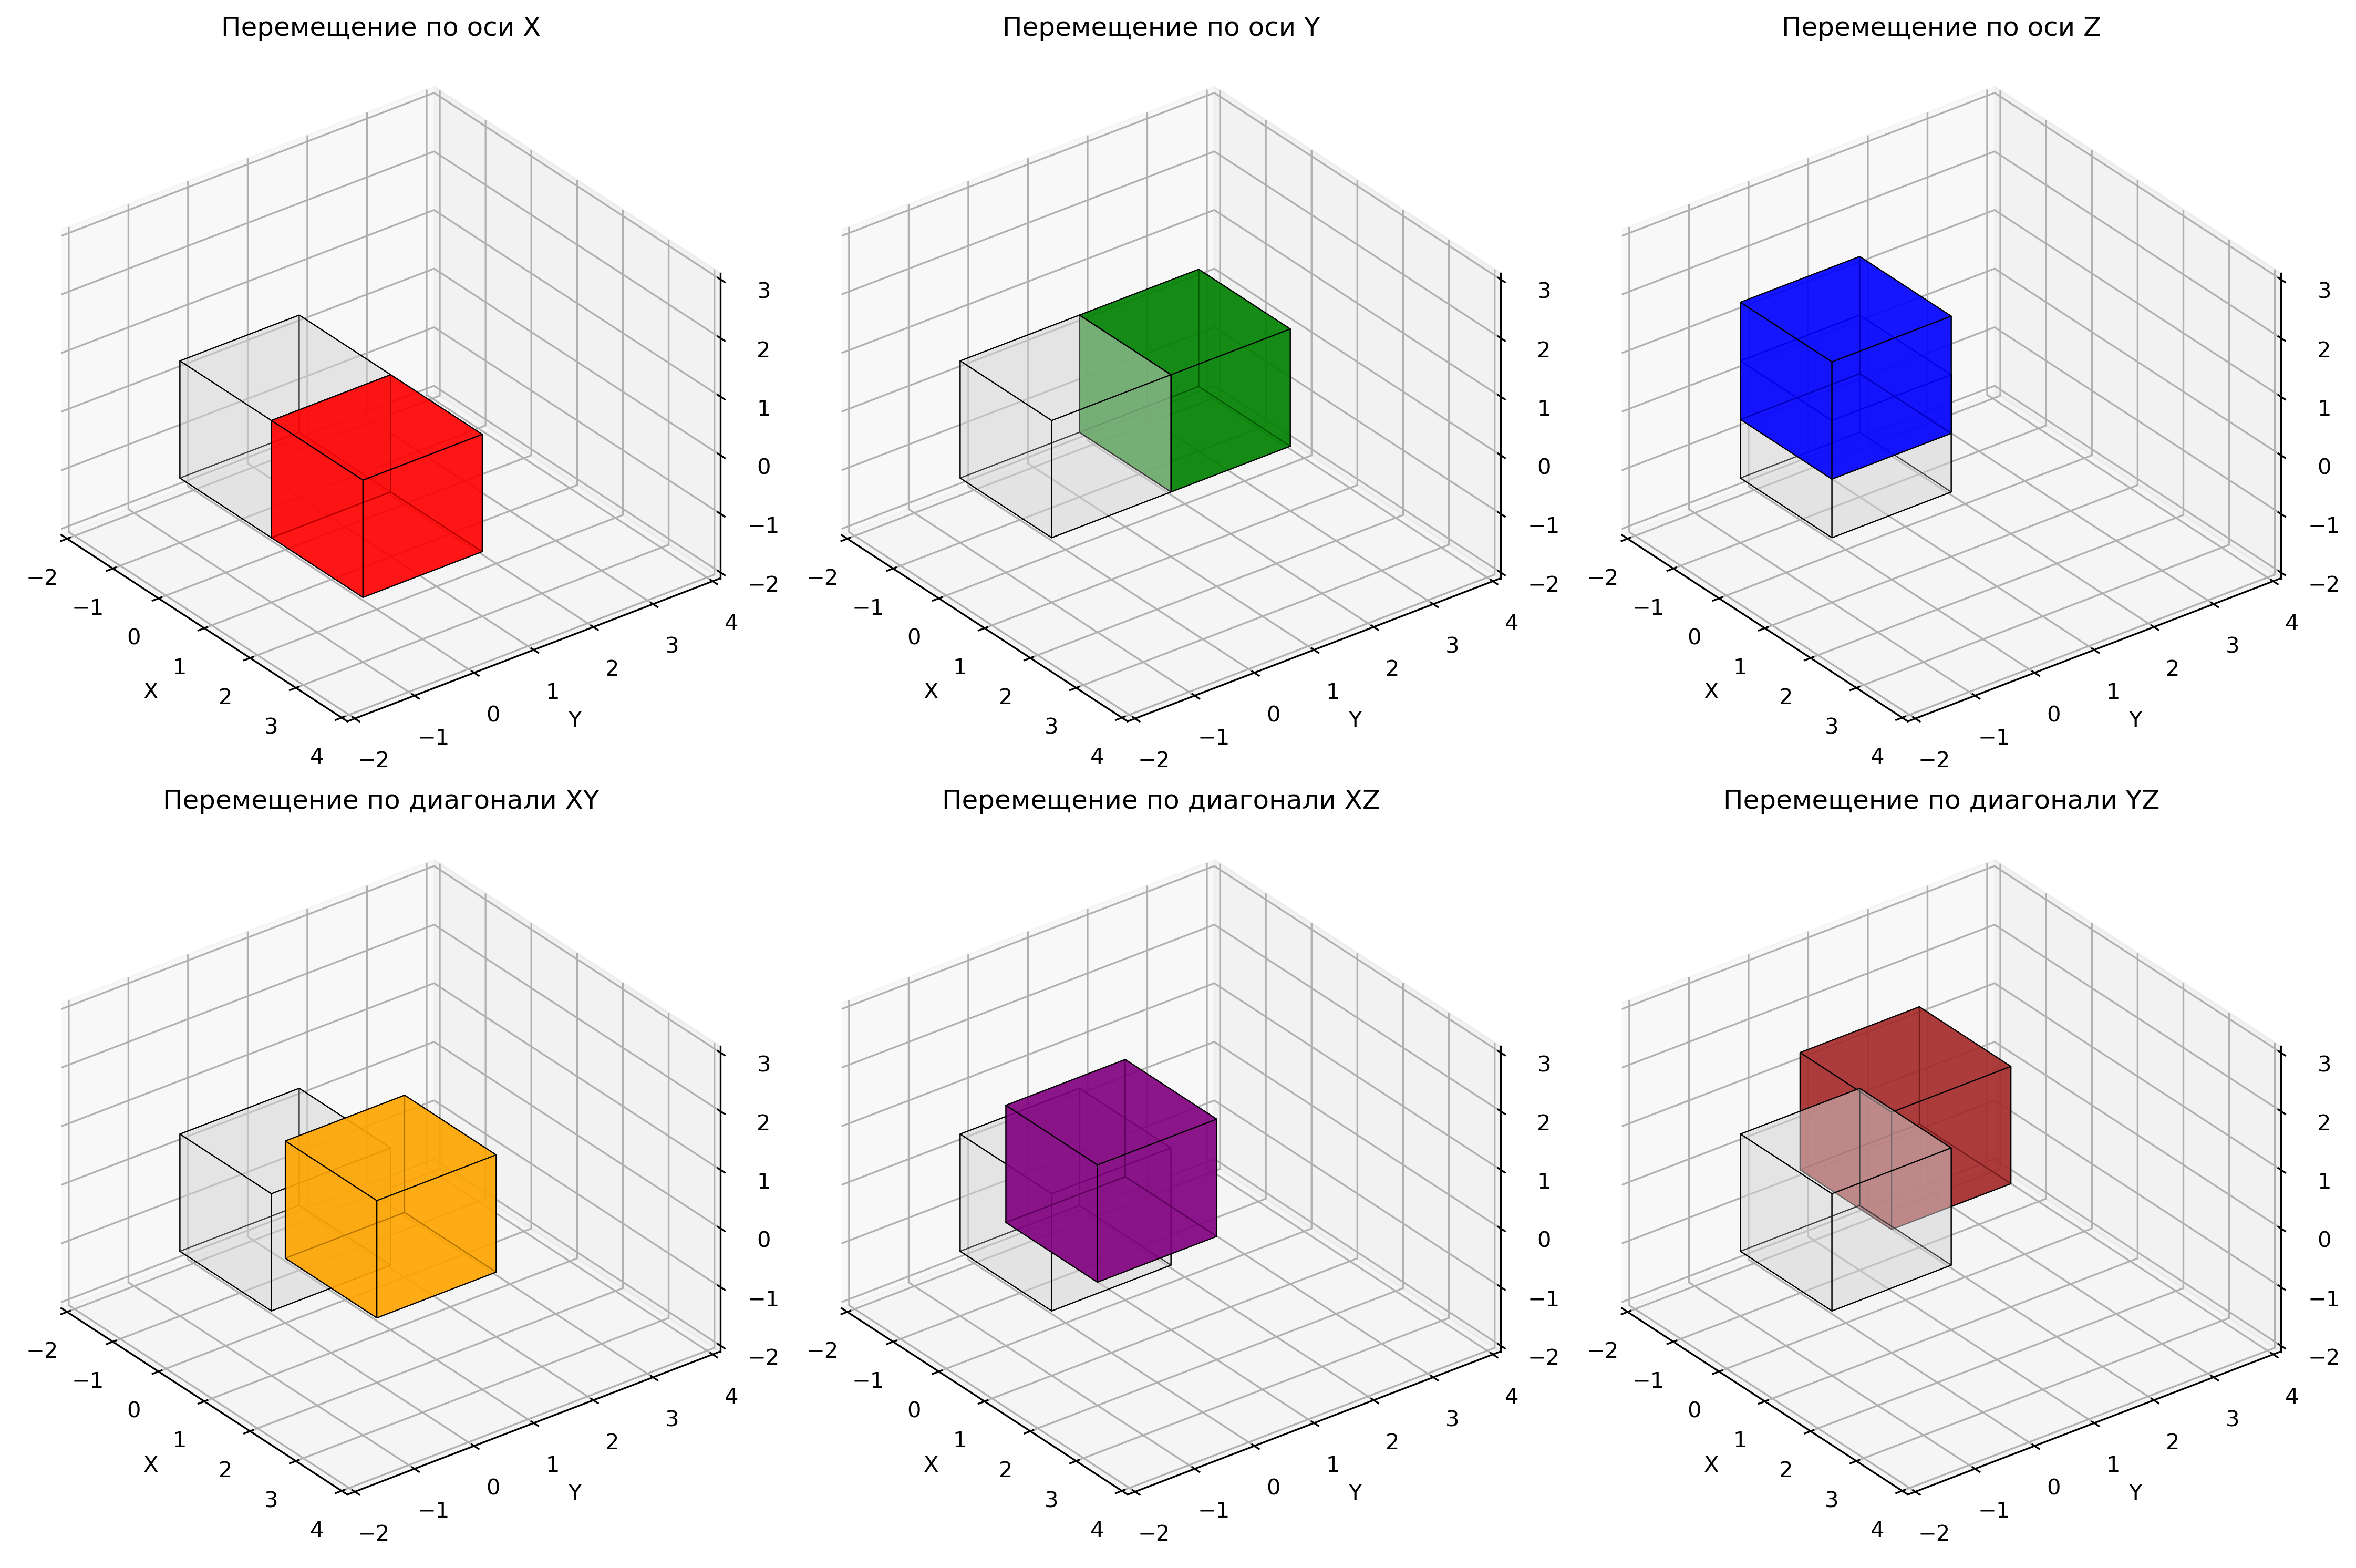
\includegraphics[width=\textwidth]{images/task3/translation_transformations.png}
\caption{Различные виды перемещения кубика}
\label{fig:translation_transformations}
\end{figure}

\subsection*{Сравнение TS и ST для перемещения}

\begin{figure}[h]
\centering
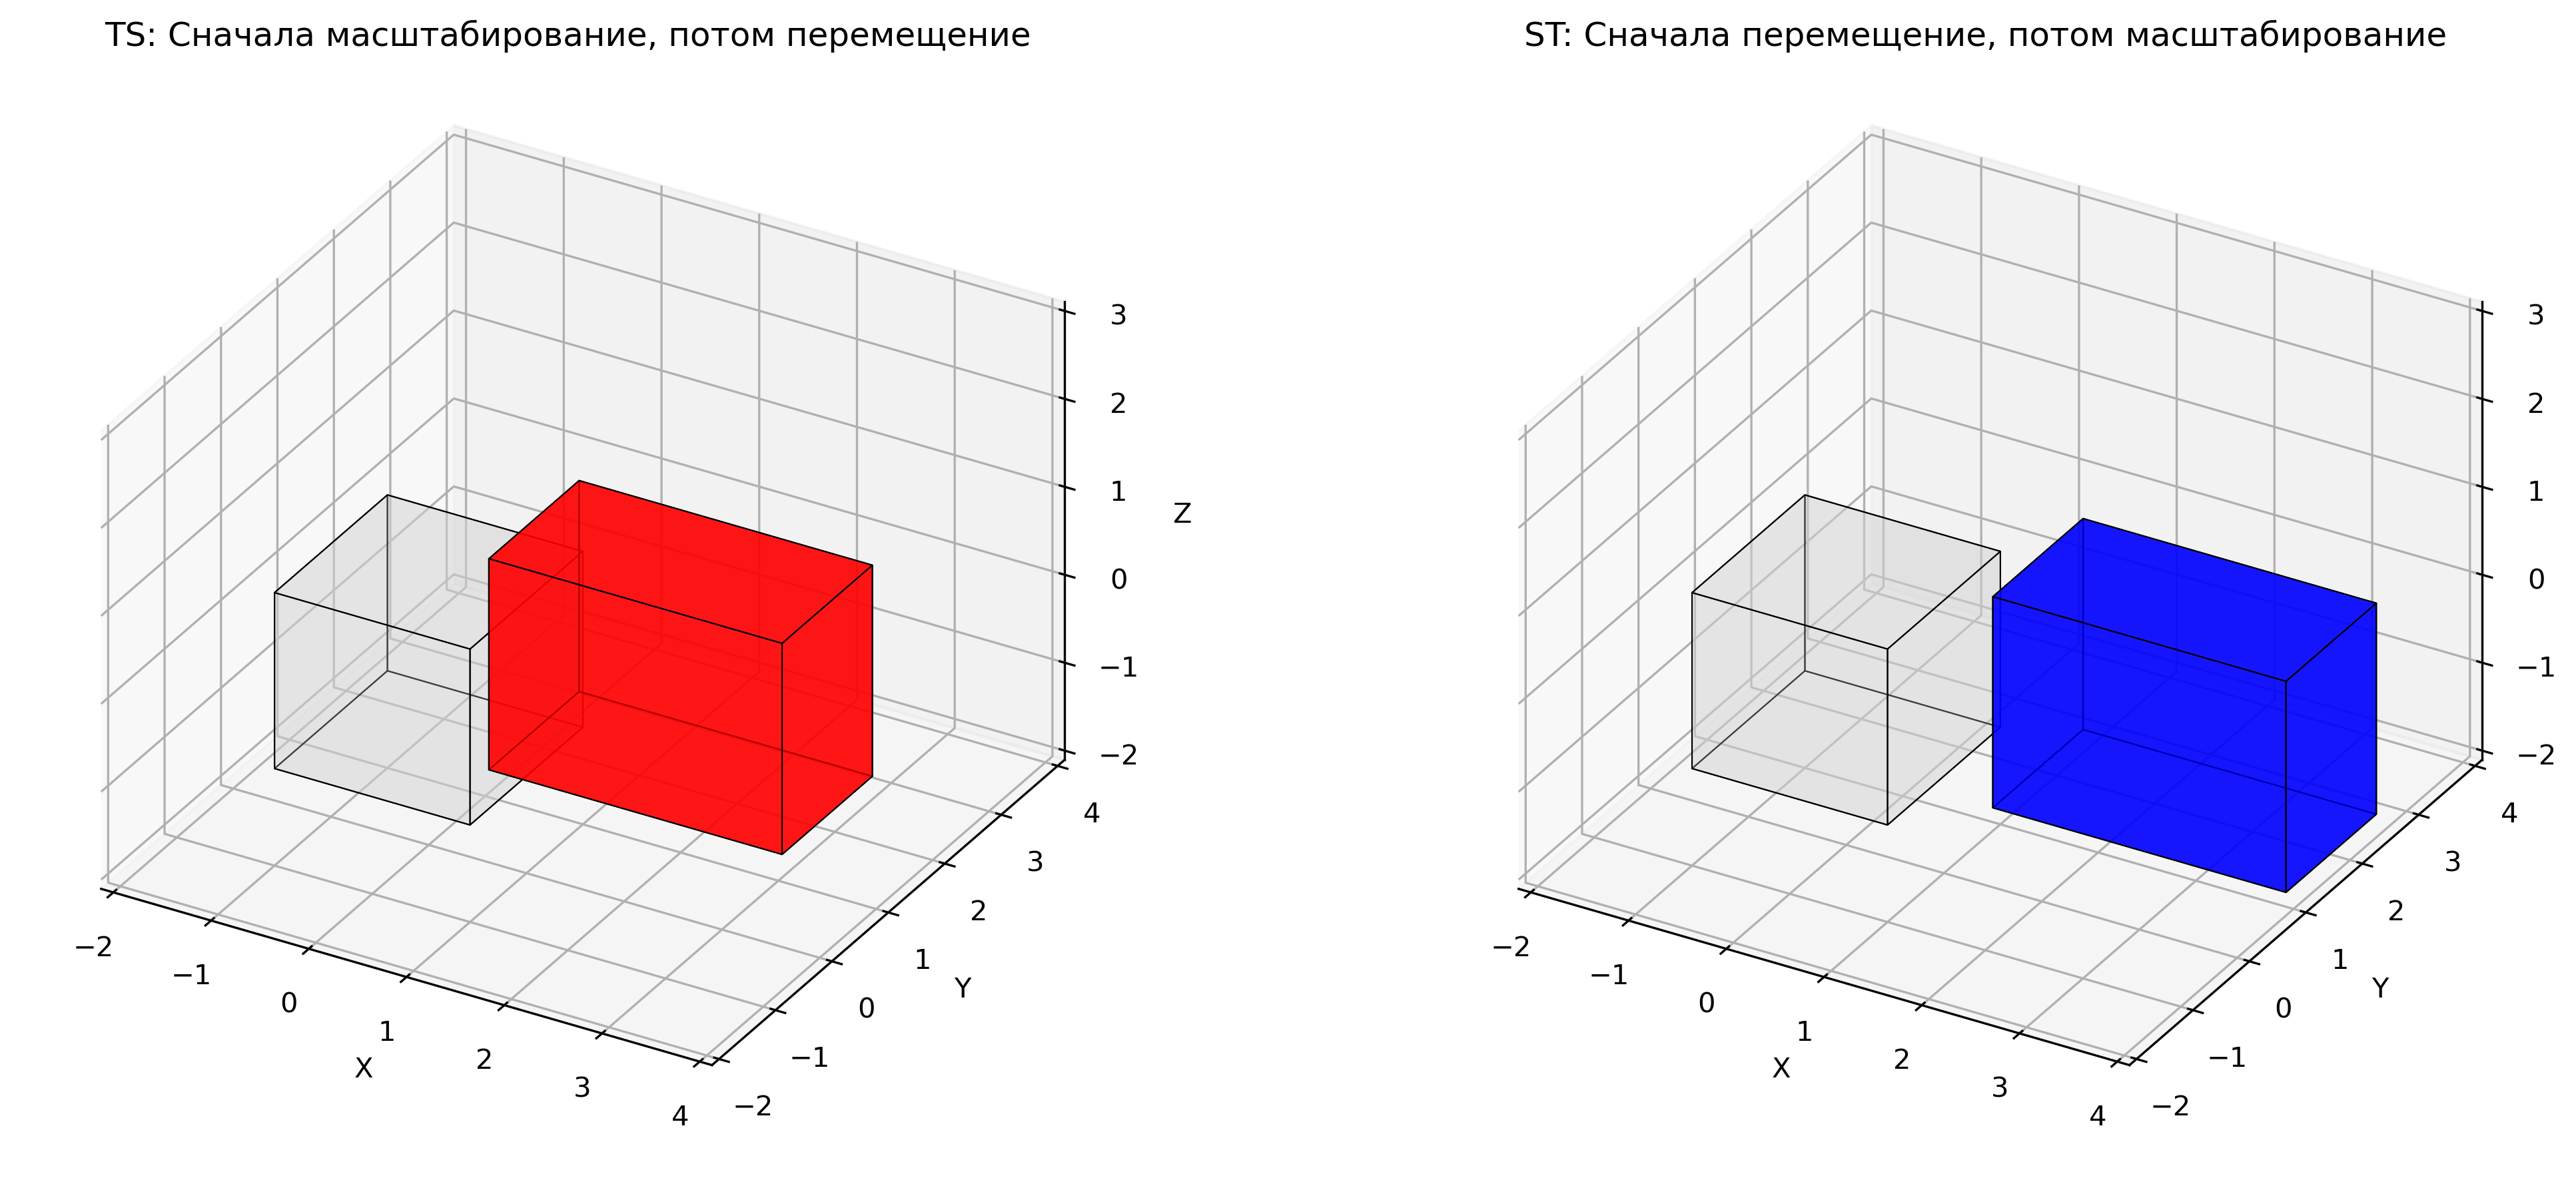
\includegraphics[width=\textwidth]{images/task3/TS_vs_ST_translation.png}
\caption{Сравнение преобразований TS и ST для перемещения}
\label{fig:TS_vs_ST_translation}
\end{figure}

\section*{Задание 4: Вращение кубика}

\subsection*{Вращение вокруг произвольной оси}

Для вращения вокруг произвольной оси $\mathbf{v} = [v_x, v_y, v_z]$ на угол $\theta$ используется формула:

\begin{equation}
\mathbf{v} = \begin{bmatrix} v_x \\ v_y \\ v_z \end{bmatrix}, \quad
J = \frac{1}{\|\mathbf{v}\|} \begin{bmatrix}
0 & -v_z & v_y & 0 \\
v_z & 0 & -v_x & 0 \\
-v_y & v_x & 0 & 0 \\
0 & 0 & 0 & 0
\end{bmatrix}
\end{equation}

\begin{equation}
R_{\mathbf{v}}(\theta) = e^{J\theta}
\end{equation}

\subsection*{Матрицы вращения вокруг координатных осей}

При выборе вектора $\mathbf{v}$ вдоль осей координат получаем стандартные матрицы вращения:

\begin{equation}
R_x(\theta) = \begin{bmatrix}
1 & 0 & 0 & 0 \\
0 & \cos\theta & -\sin\theta & 0 \\
0 & \sin\theta & \cos\theta & 0 \\
0 & 0 & 0 & 1
\end{bmatrix}
\end{equation}

\begin{equation}
R_y(\phi) = \begin{bmatrix}
\cos\phi & 0 & \sin\phi & 0 \\
0 & 1 & 0 & 0 \\
-\sin\phi & 0 & \cos\phi & 0 \\
0 & 0 & 0 & 1
\end{bmatrix}
\end{equation}

\begin{equation}
R_z(\psi) = \begin{bmatrix}
\cos\psi & -\sin\psi & 0 & 0 \\
\sin\psi & \cos\psi & 0 & 0 \\
0 & 0 & 1 & 0 \\
0 & 0 & 0 & 1
\end{bmatrix}
\end{equation}

\subsection*{Теорема вращения Эйлера}

Любое вращение в 3D-пространстве можно представить как композицию трех вращений вокруг координатных осей:

\begin{equation}
R = R_x(\theta) R_y(\phi) R_z(\psi)
\end{equation}

Однако это представление не является единственным и может привести к проблеме "карданного подвеса" (gimbal lock).

\subsection*{Достаточность композиции вращений}

Композиция $R_x(\theta) R_y(\phi) R_z(\psi)$ \textbf{не является достаточной} для описания всех возможных вращений в 3D-пространстве. Проблемы:

\begin{enumerate}
\item \textbf{Карданный подвес}: При $\phi = \pm \frac{\pi}{2}$ теряется одна степень свободы
\item \textbf{Неединственность}: Одно и то же вращение может быть представлено разными наборами углов
\item \textbf{Сингулярности}: При определенных углах возникают проблемы с численной стабильностью
\end{enumerate}

\subsection*{Восстановление оси вращения}

Ось вращения \textbf{может быть восстановлена} из матрицы вращения $R$:

\begin{enumerate}
\item Вычислить след матрицы: $\text{tr}(R) = 1 + 2\cos\theta$
\item Найти угол вращения: $\theta = \arccos\left(\frac{\text{tr}(R) - 1}{2}\right)$
\item Вычислить ось вращения: $\mathbf{v} = \frac{1}{2\sin\theta} \begin{bmatrix} R_{32} - R_{23} \\ R_{13} - R_{31} \\ R_{21} - R_{12} \end{bmatrix}$
\end{enumerate}

Это возможно благодаря тому, что любое вращение в 3D имеет неподвижную ось (теорема Эйлера).

\begin{figure}[h]
\centering
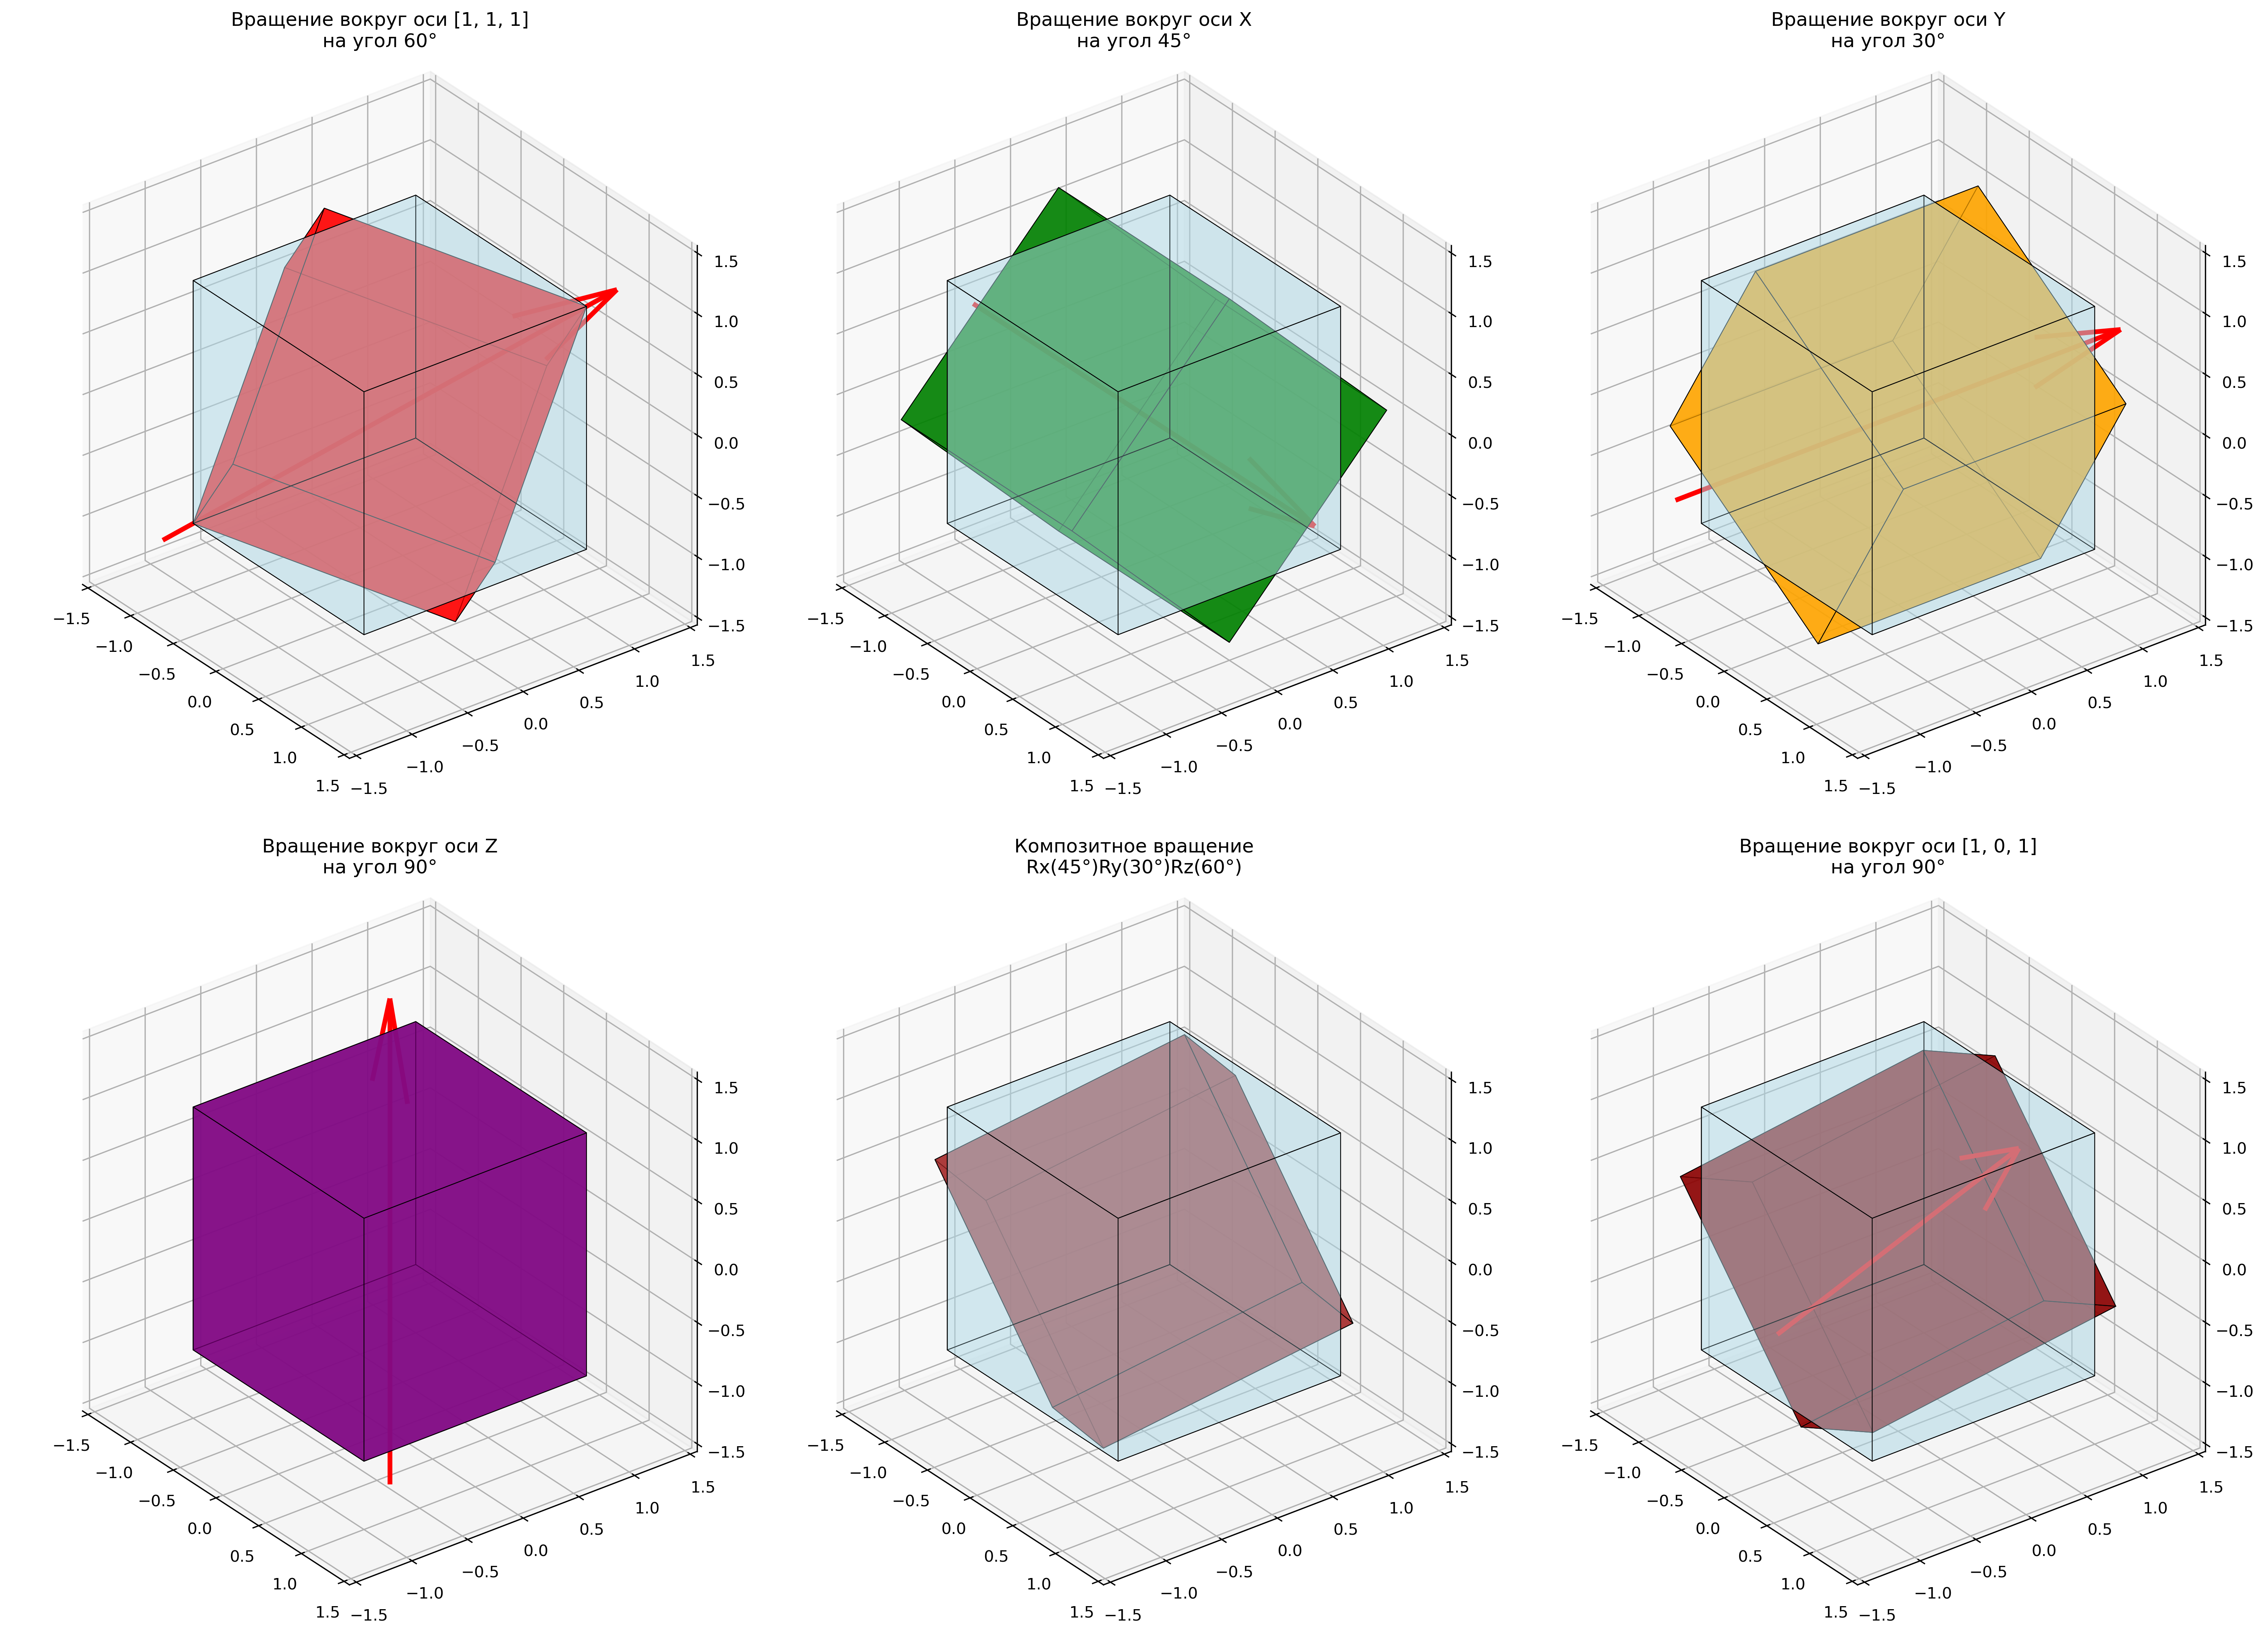
\includegraphics[width=\textwidth]{images/task4/rotation_transformations.png}
\caption{Вращения кубика вокруг различных осей}
\label{fig:rotation_transformations}
\end{figure}

\subsection*{Сравнение формул вращения}

\begin{figure}[h]
\centering
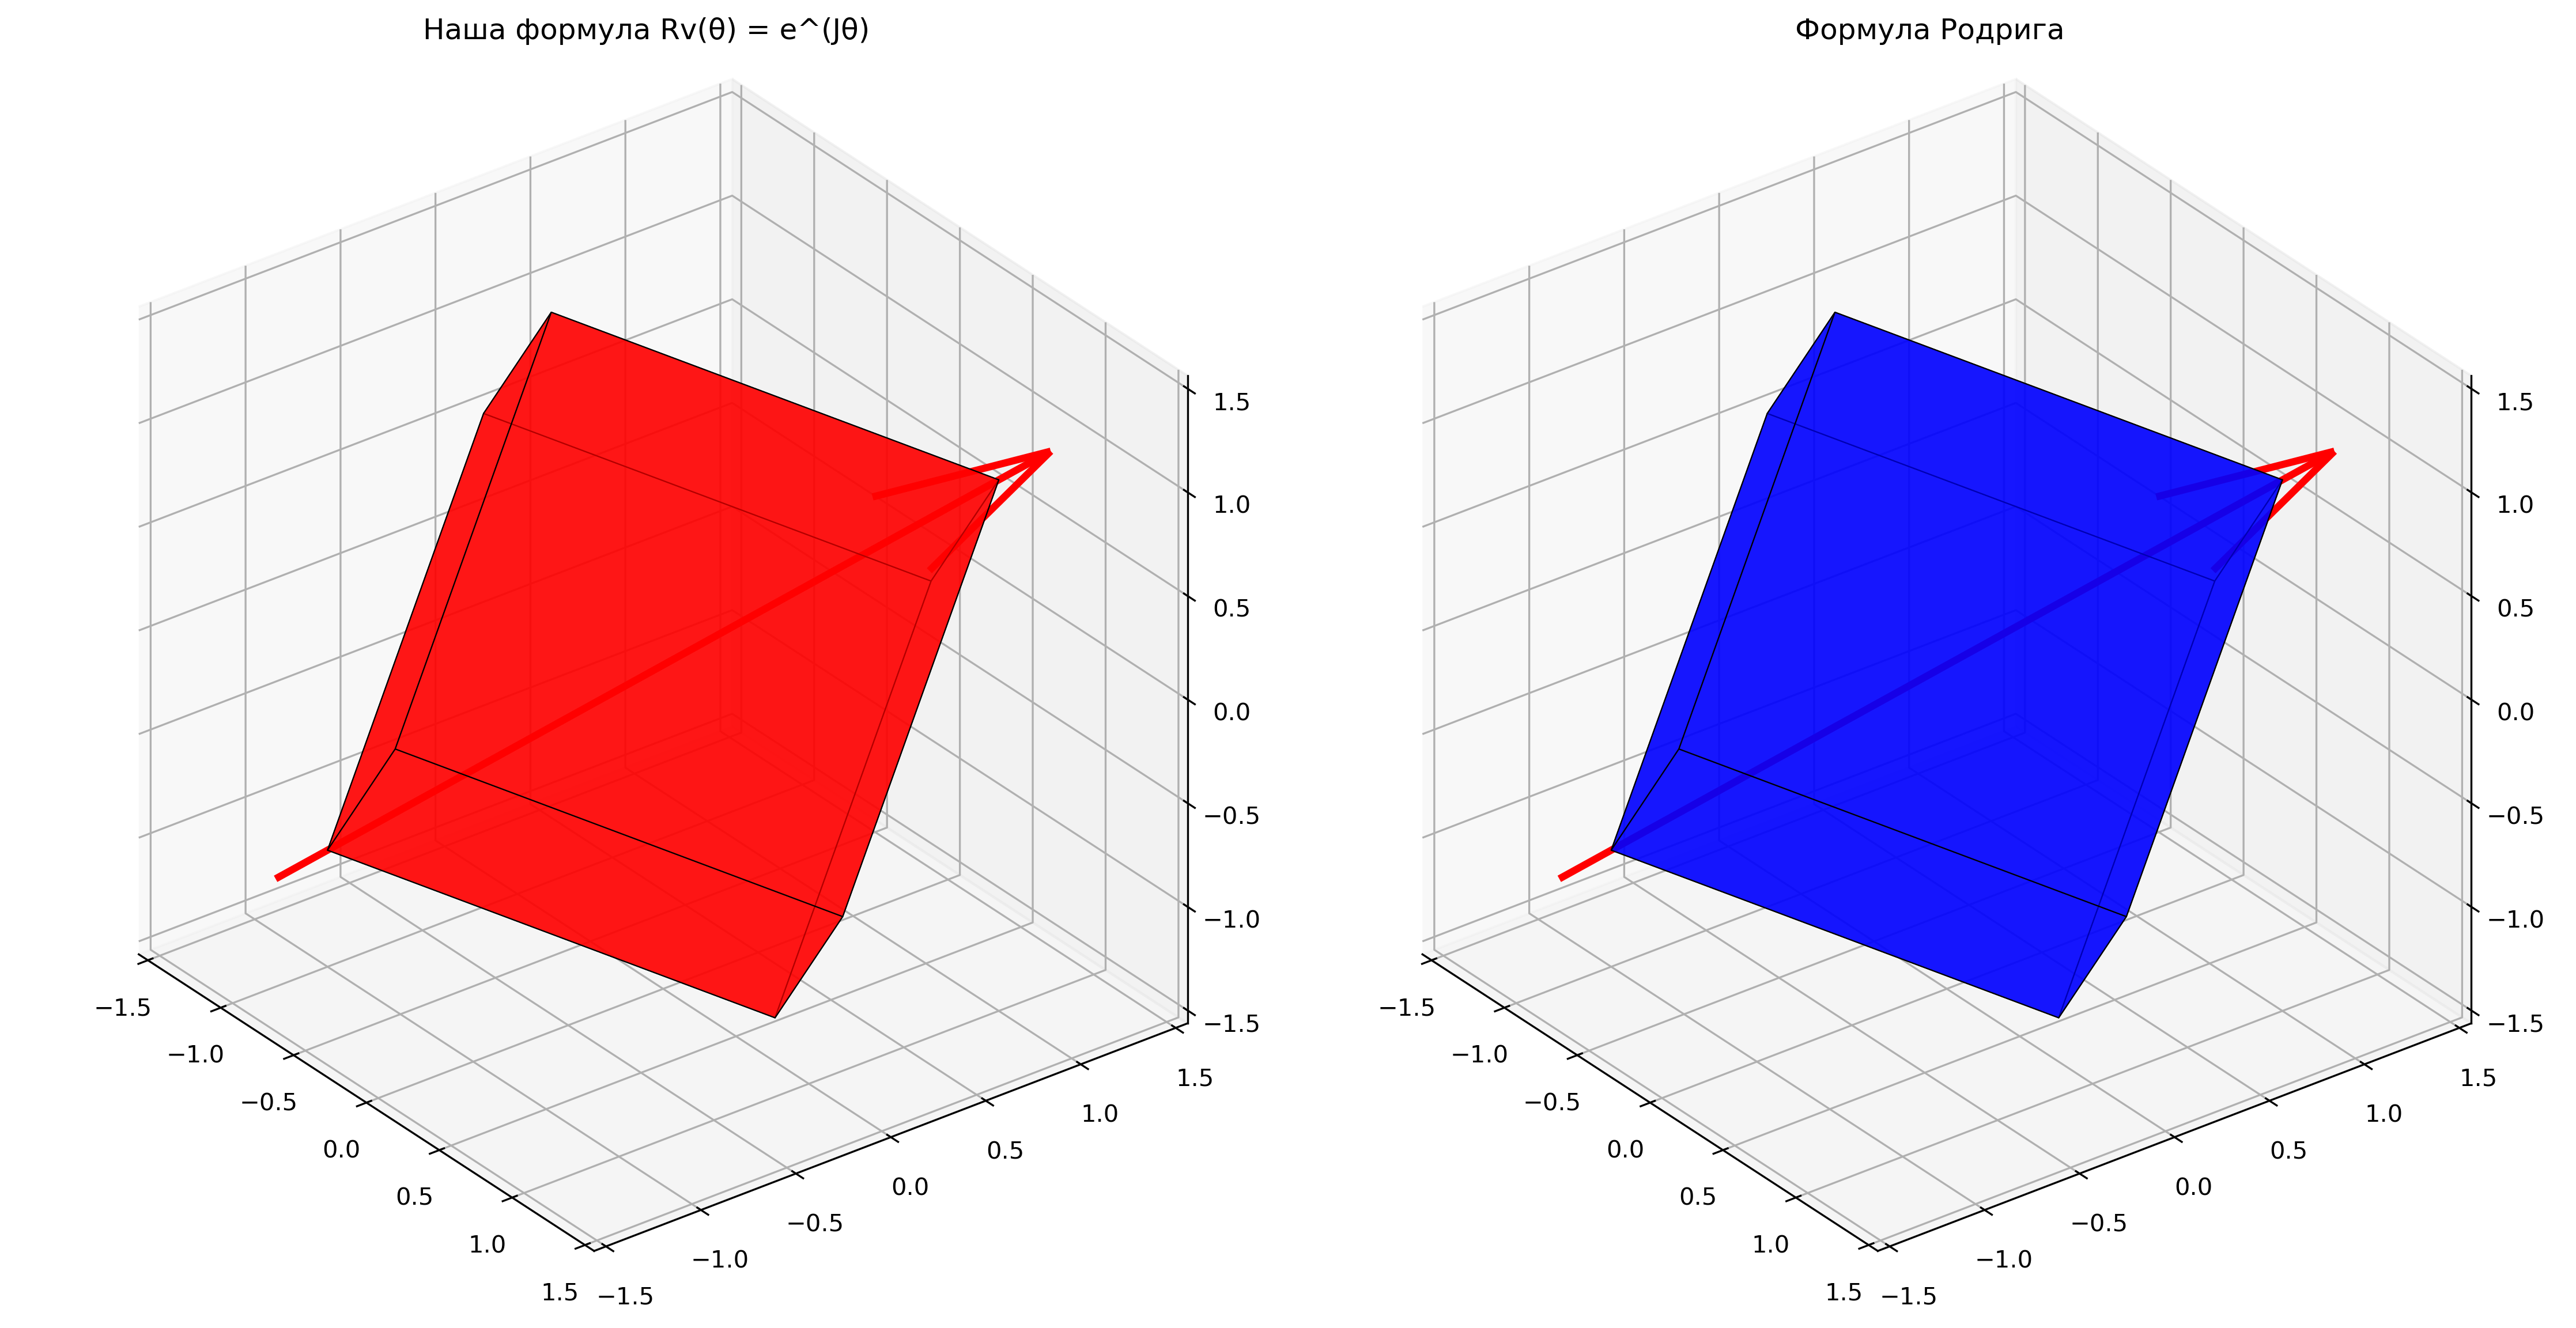
\includegraphics[width=\textwidth]{images/task4/rotation_formula_comparison.png}
\caption{Сравнение формулы $R_{\mathbf{v}}(\theta) = e^{J\theta}$ с формулой Родрига}
\label{fig:rotation_formula_comparison}
\end{figure}

\section*{Задание 5: Вращение вокруг вершины}

\subsection*{Алгоритм вращения вокруг точки}

Для вращения объекта вокруг произвольной точки $P = (p_x, p_y, p_z)$ используется композиция преобразований:

\begin{enumerate}
\item Перенос точки $P$ в начало координат: $T_1 = T(-p_x, -p_y, -p_z)$
\item Вращение вокруг оси: $R = R_{\mathbf{v}}(\theta)$
\item Обратный перенос: $T_2 = T(p_x, p_y, p_z)$
\end{enumerate}

Итоговая матрица преобразования:
\begin{equation}
M = T_2 \cdot R \cdot T_1
\end{equation}

\begin{figure}[h]
\centering
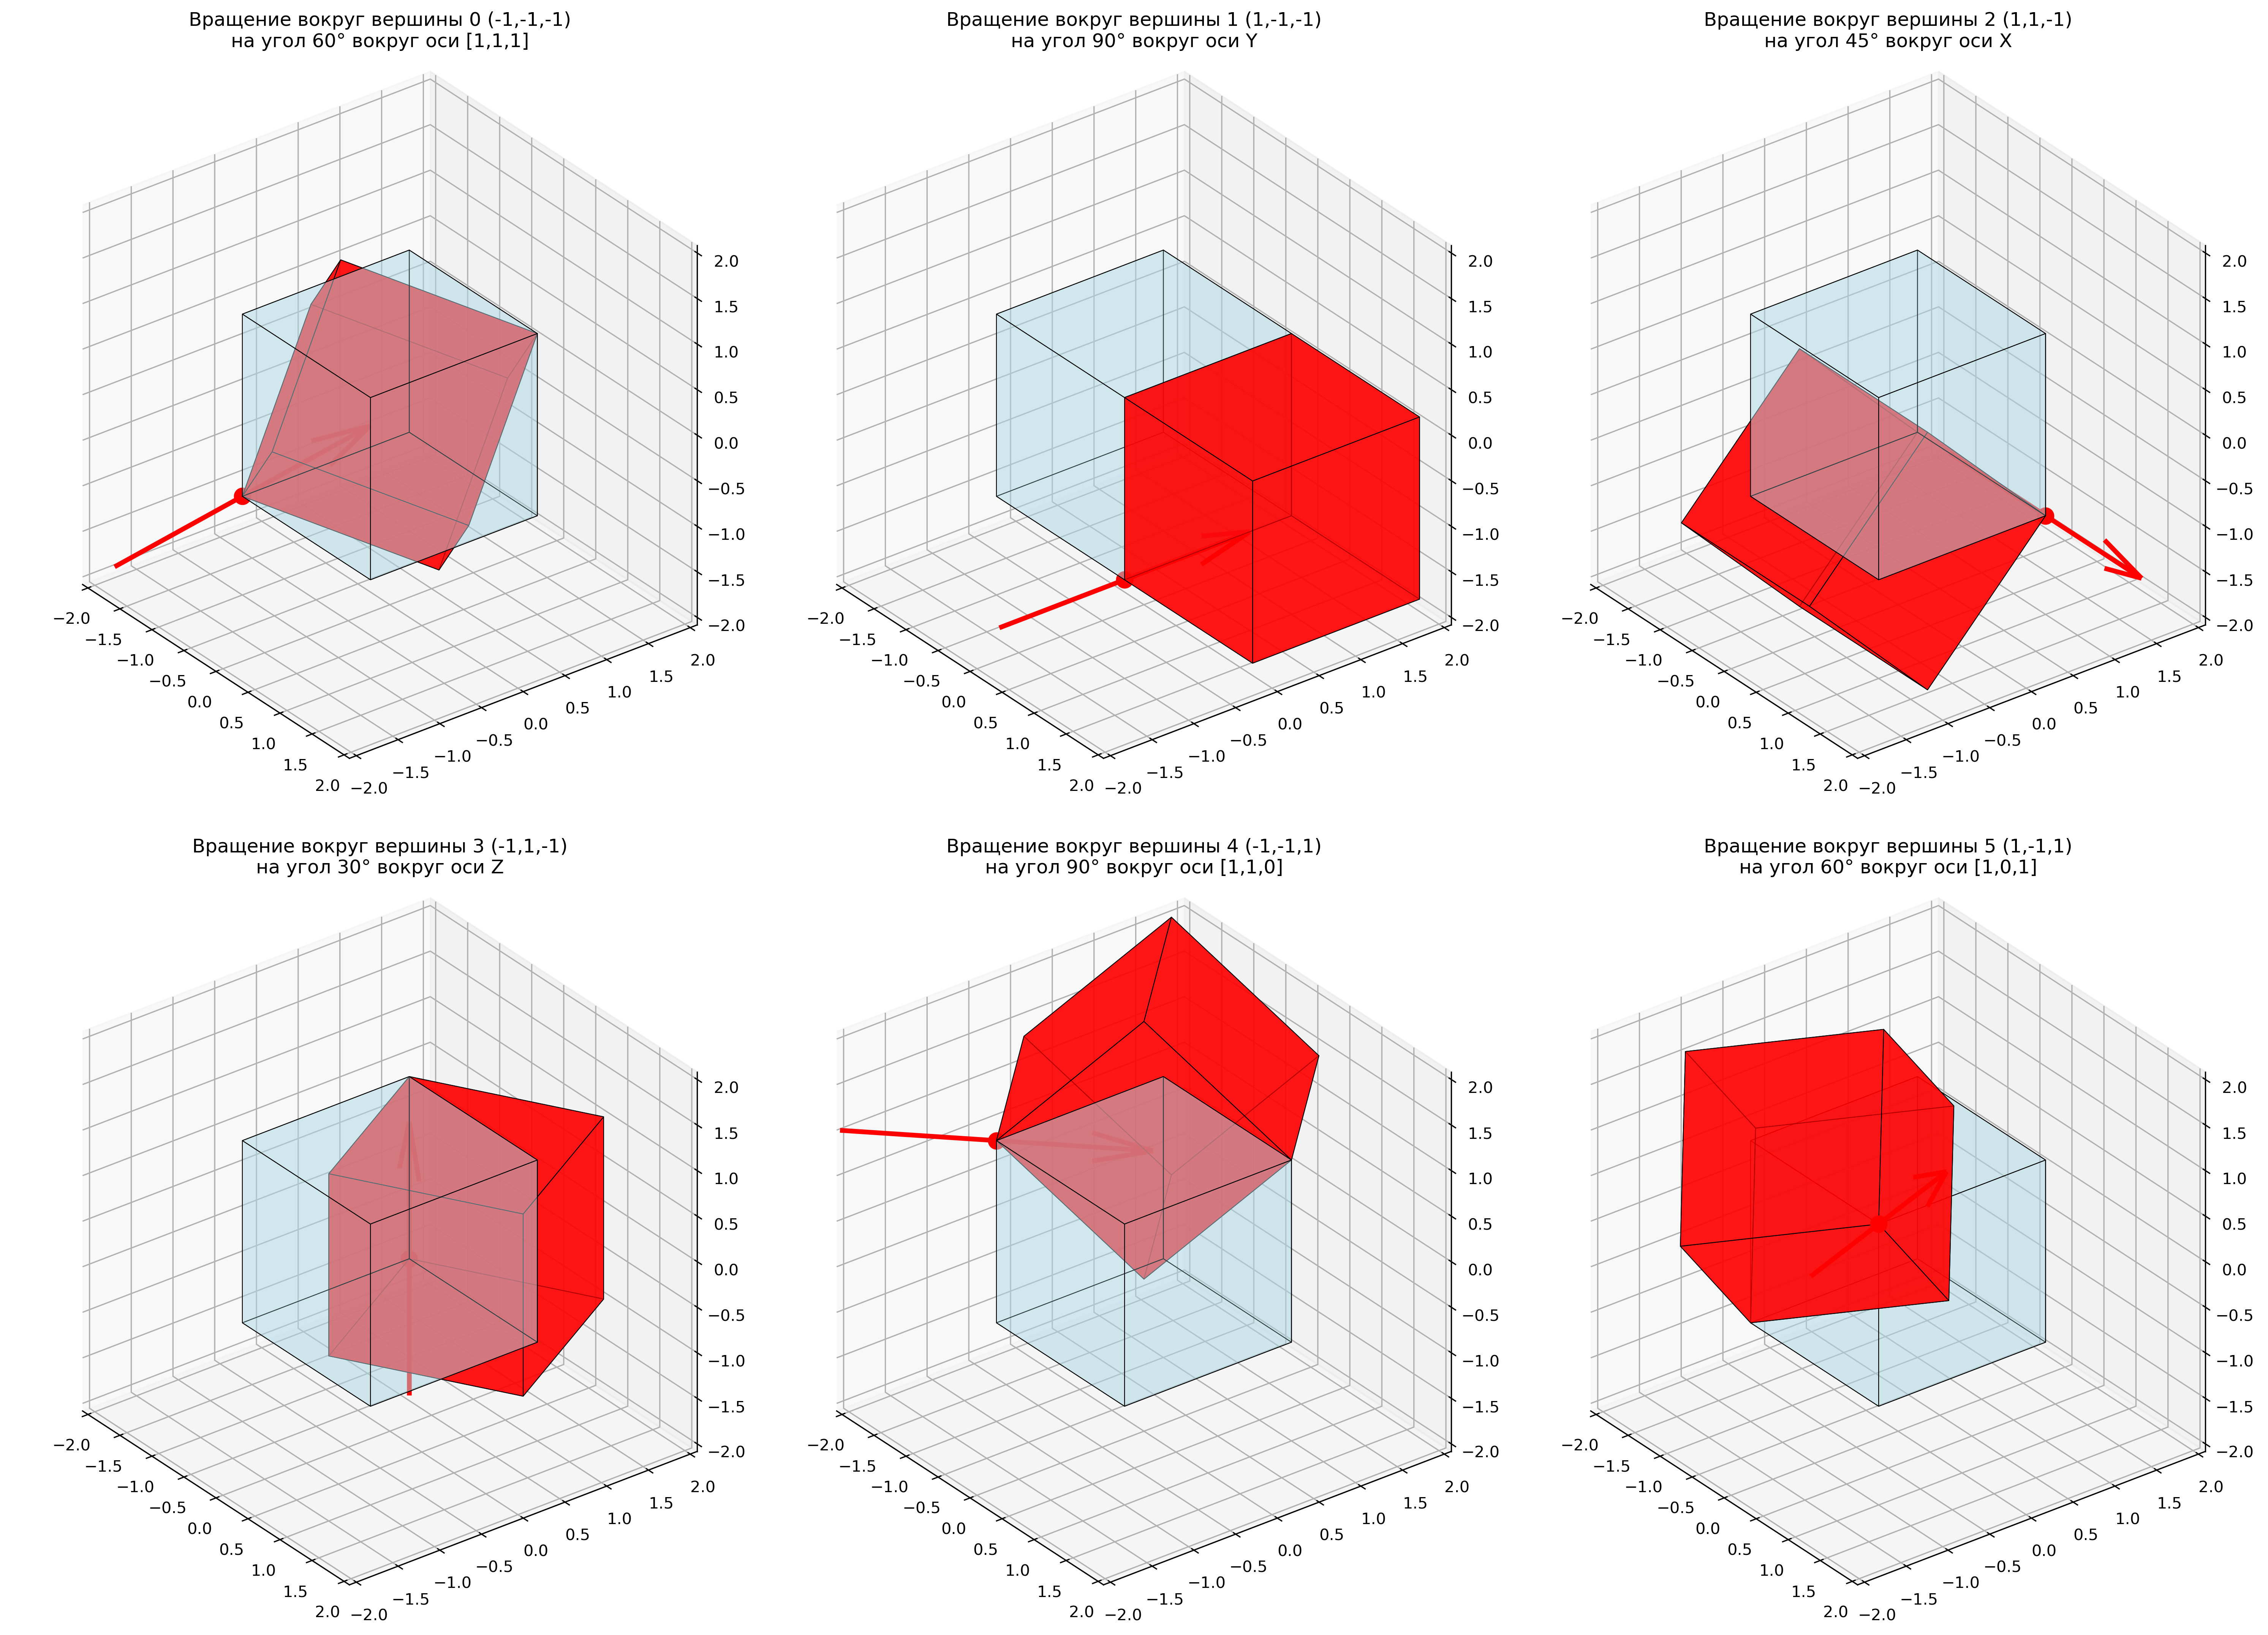
\includegraphics[width=\textwidth]{images/task5/rotation_around_vertices.png}
\caption{Вращения кубика вокруг различных вершин}
\label{fig:rotation_around_vertices}
\end{figure}

\subsection*{Практическая реализация}

\begin{figure}[h]
\centering
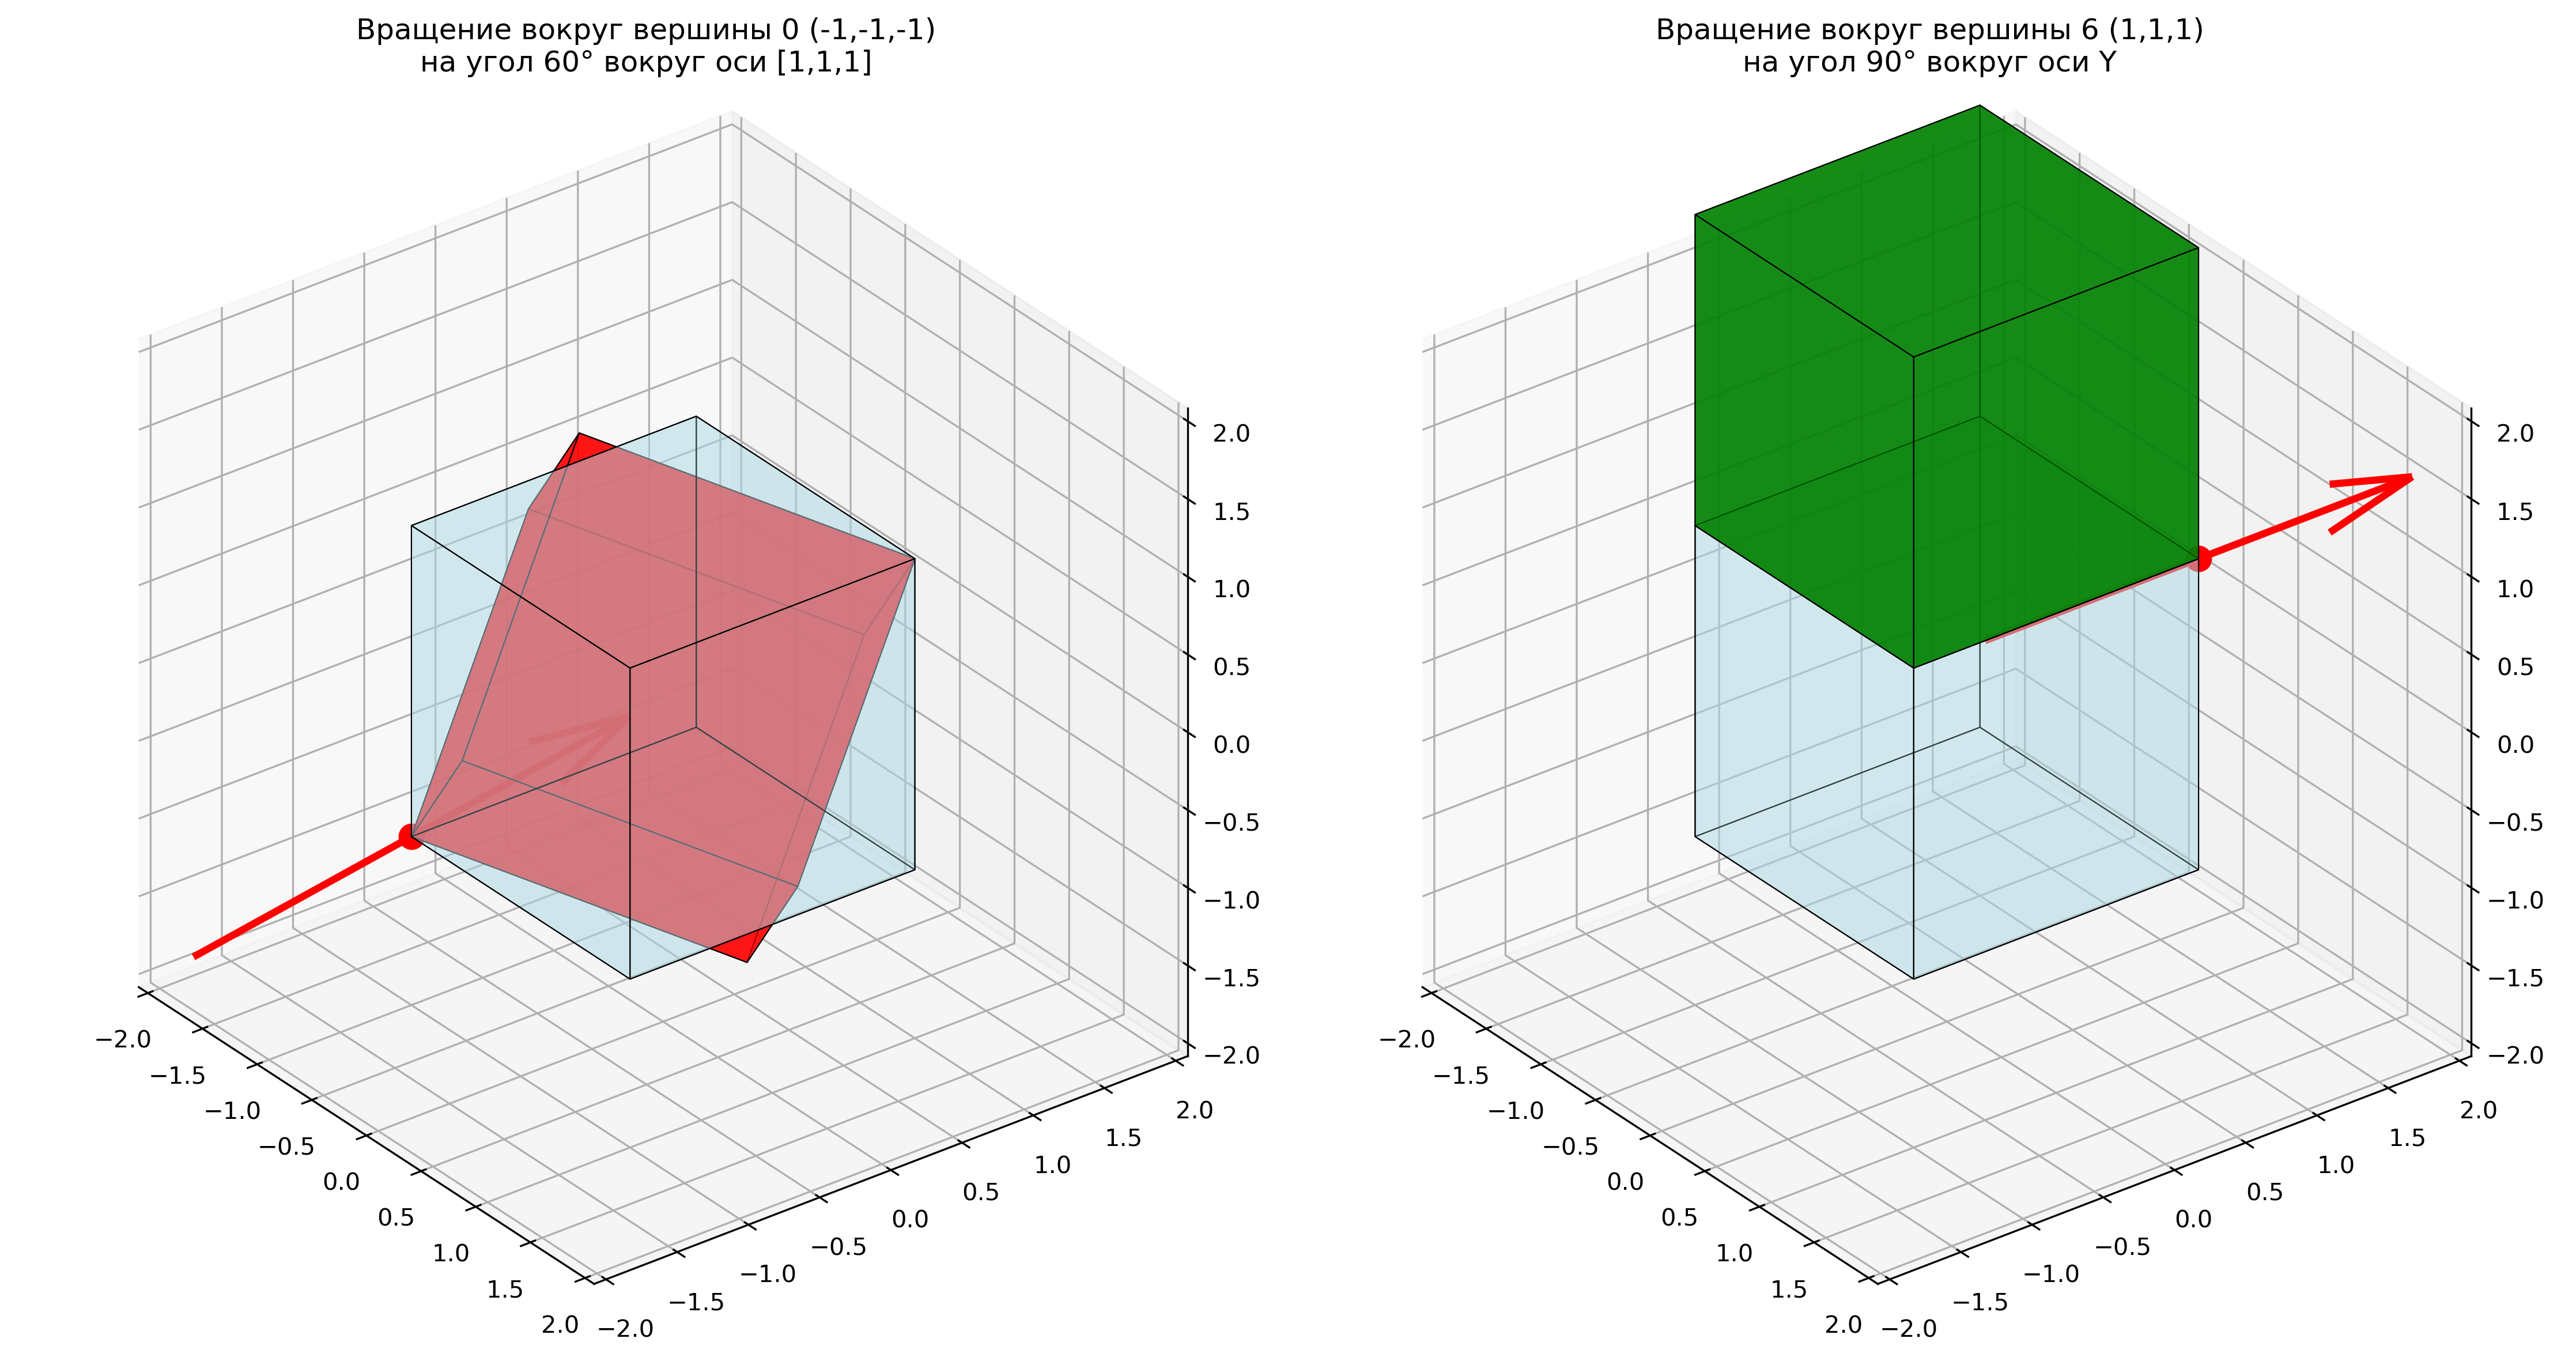
\includegraphics[width=\textwidth]{images/task5/vertex_rotation_comparison.png}
\caption{Сравнение вращений вокруг разных вершин}
\label{fig:vertex_rotation_comparison}
\end{figure}

\section*{Задание 6: Реализация камеры}

\subsection*{Матрица вида (View Matrix)}

Матрица камеры $C$ создается следующим образом:

\begin{enumerate}
\item Вычисление вектора направления камеры: $\mathbf{forward} = \frac{\mathbf{target} - \mathbf{position}}{\|\mathbf{target} - \mathbf{position}\|}$
\item Вычисление правого вектора: $\mathbf{right} = \frac{\mathbf{forward} \times \mathbf{up}}{\|\mathbf{forward} \times \mathbf{up}\|}$
\item Вычисление вектора "вверх": $\mathbf{up} = \mathbf{right} \times \mathbf{forward}$
\item Создание матрицы поворота $R$ и перемещения $T$
\item Матрица камеры: $C = R \cdot T$
\end{enumerate}

\subsection*{Эффект камеры}

Применение матрицы камеры $C$ к объектам сцены эквивалентно перемещению камеры в начало координат с стандартной ориентацией.

\subsection*{Создание сцены}

Для демонстрации работы камеры создается сцена из нескольких кубиков, расположенных в разных позициях. Используется команда \texttt{ax.view\_init(azim=0, elev=-90)} для просмотра сцены "снизу".

\subsection*{Выбор позиций камеры}

Выбираются различные позиции камеры $T_c$ и матрицы поворота $R_c(\theta)$:
\begin{itemize}
\item Камера в позиции $[5, 5, 3]$ смотрит на центр сцены
\item Камера в позиции $[-4, -4, 2]$ смотрит на центр сцены  
\item Камера в позиции $[0, 0, 8]$ (вид сверху)
\item Камера в позиции $[6, 6, 4]$ (вид под углом)
\end{itemize}

\subsection*{Обратная матрица камеры}

Находится матрица $C^{-1}$, которая перемещает камеру из выбранной позиции в начало координат с стандартной ориентацией. Применение этой матрицы ко всем объектам сцены создает эффект, как будто камера находится в начале координат.

\begin{figure}[h]
\centering
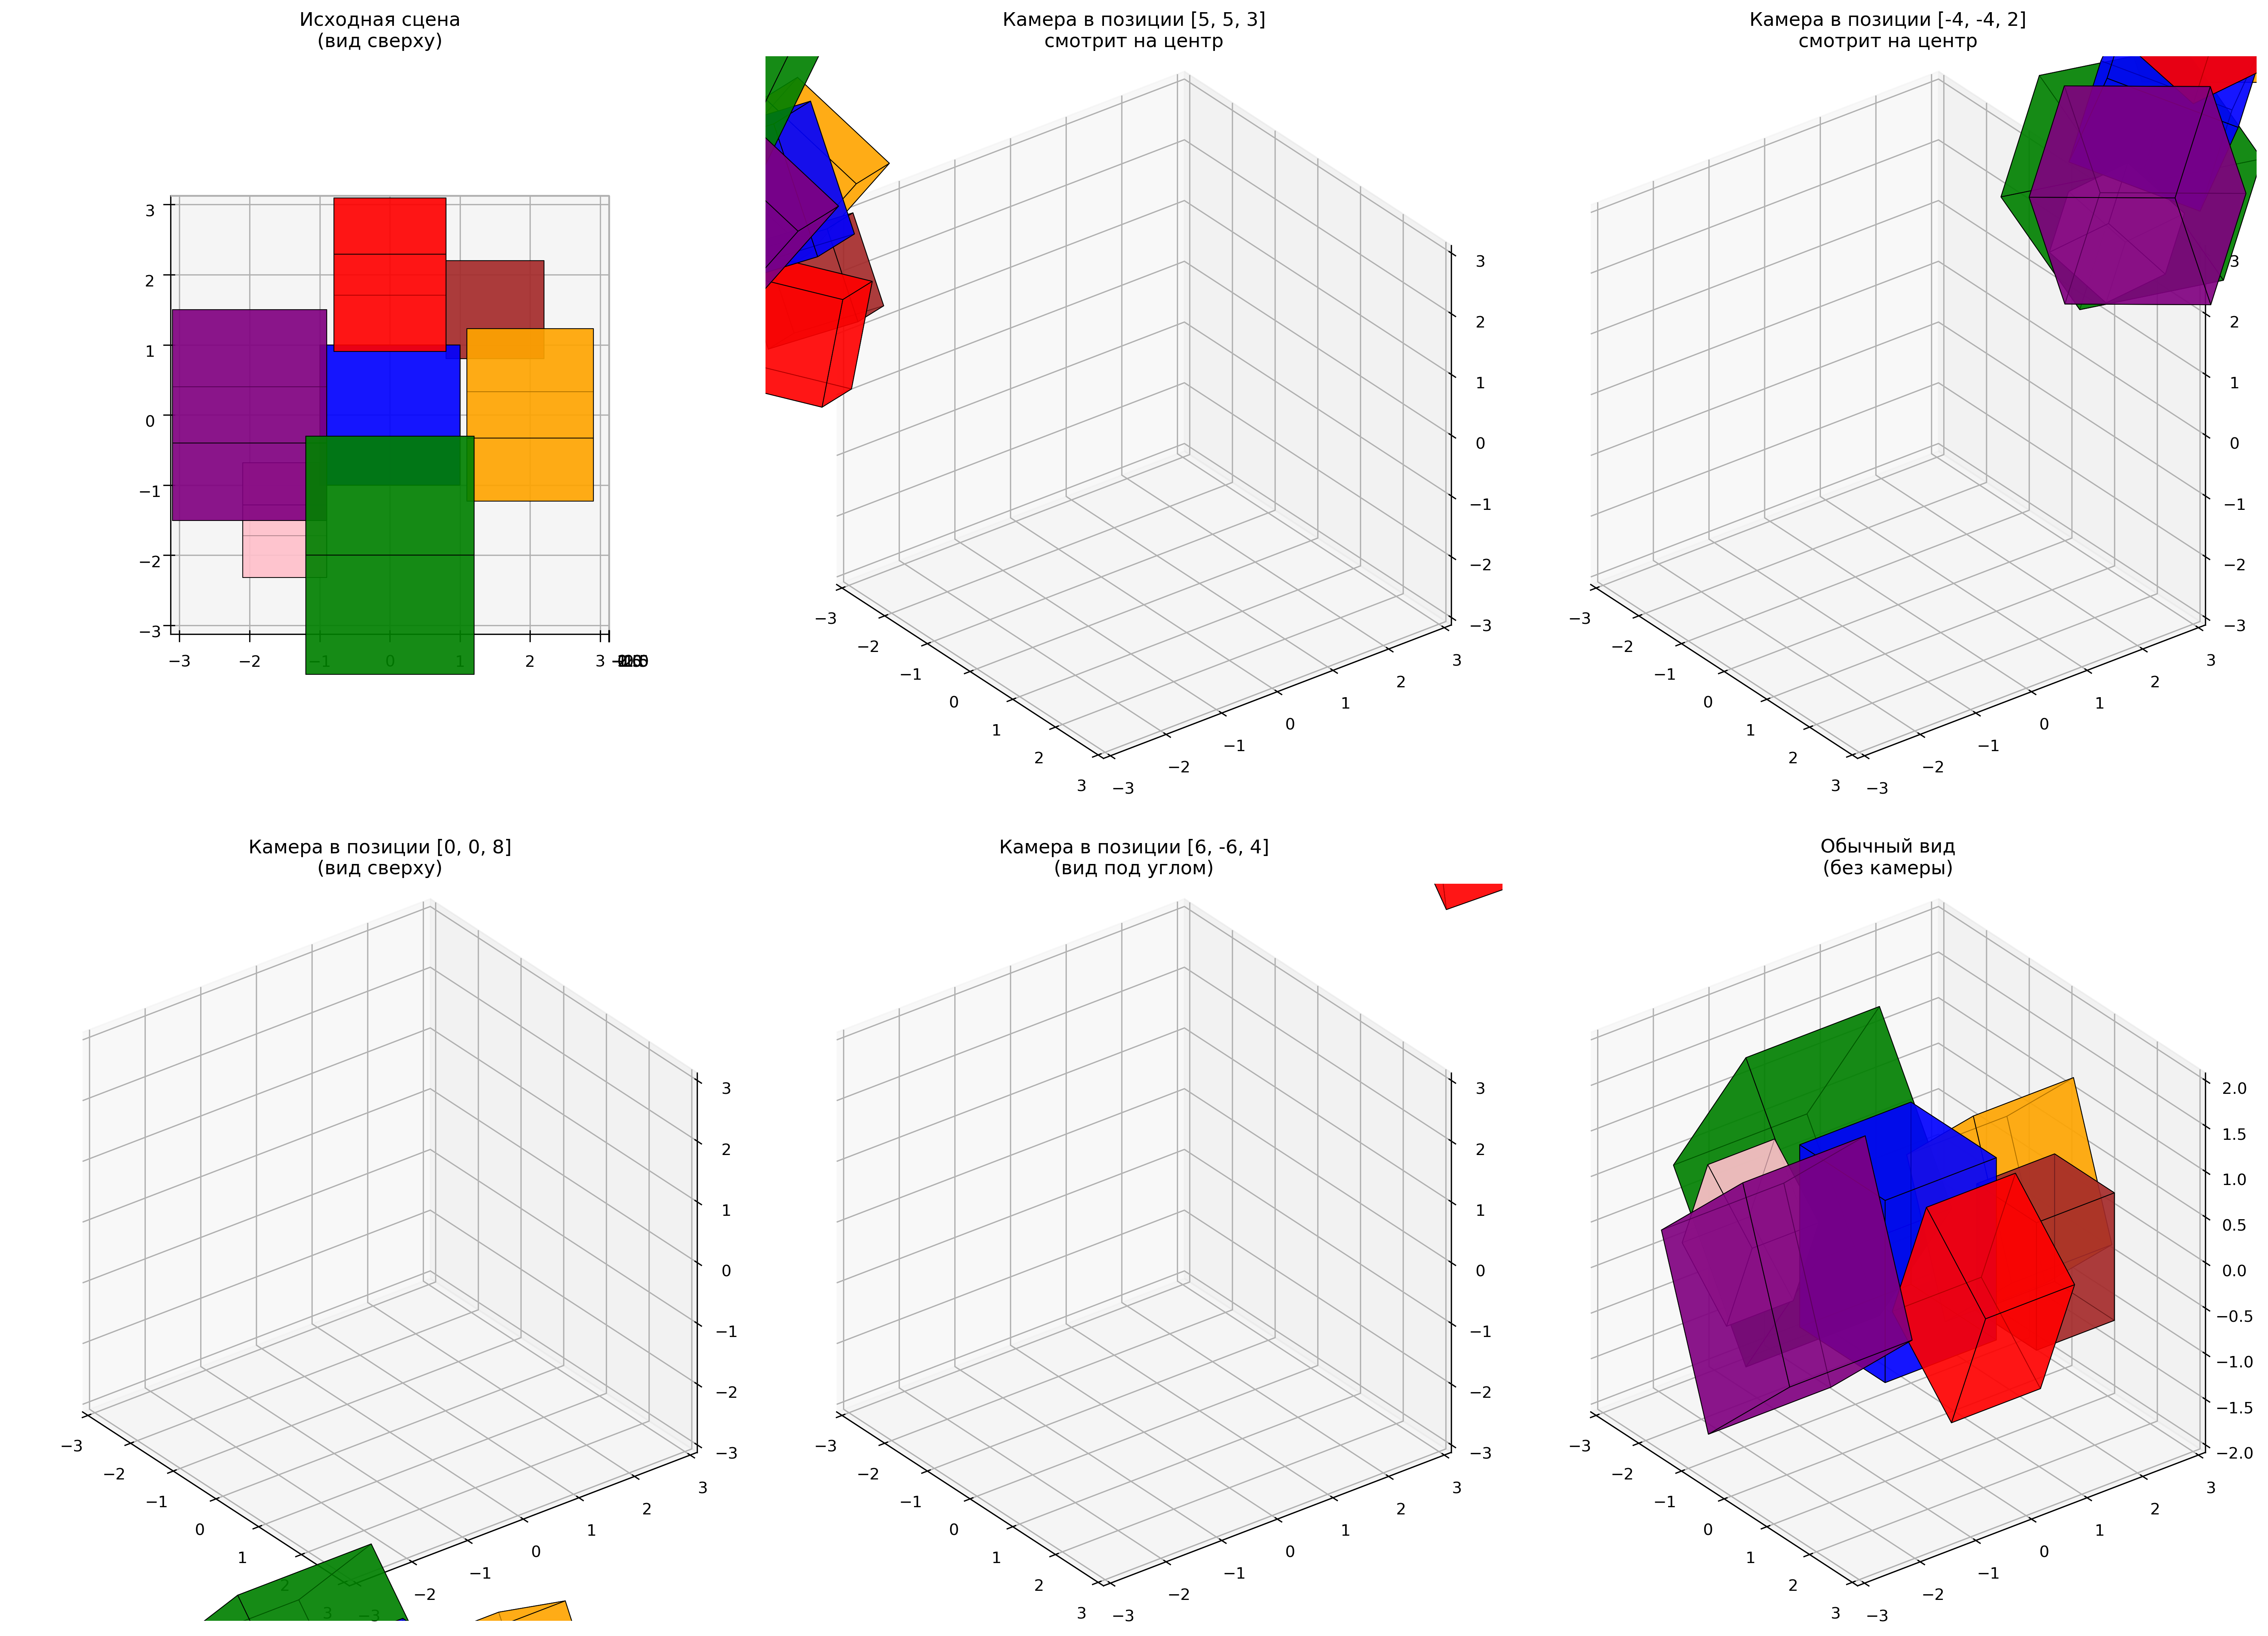
\includegraphics[width=\textwidth]{images/task6/camera_implementations.png}
\caption{Реализация камеры с различными позициями}
\label{fig:camera_implementations}
\end{figure}

\subsection*{Сравнение эффектов}

\begin{figure}[h]
\centering
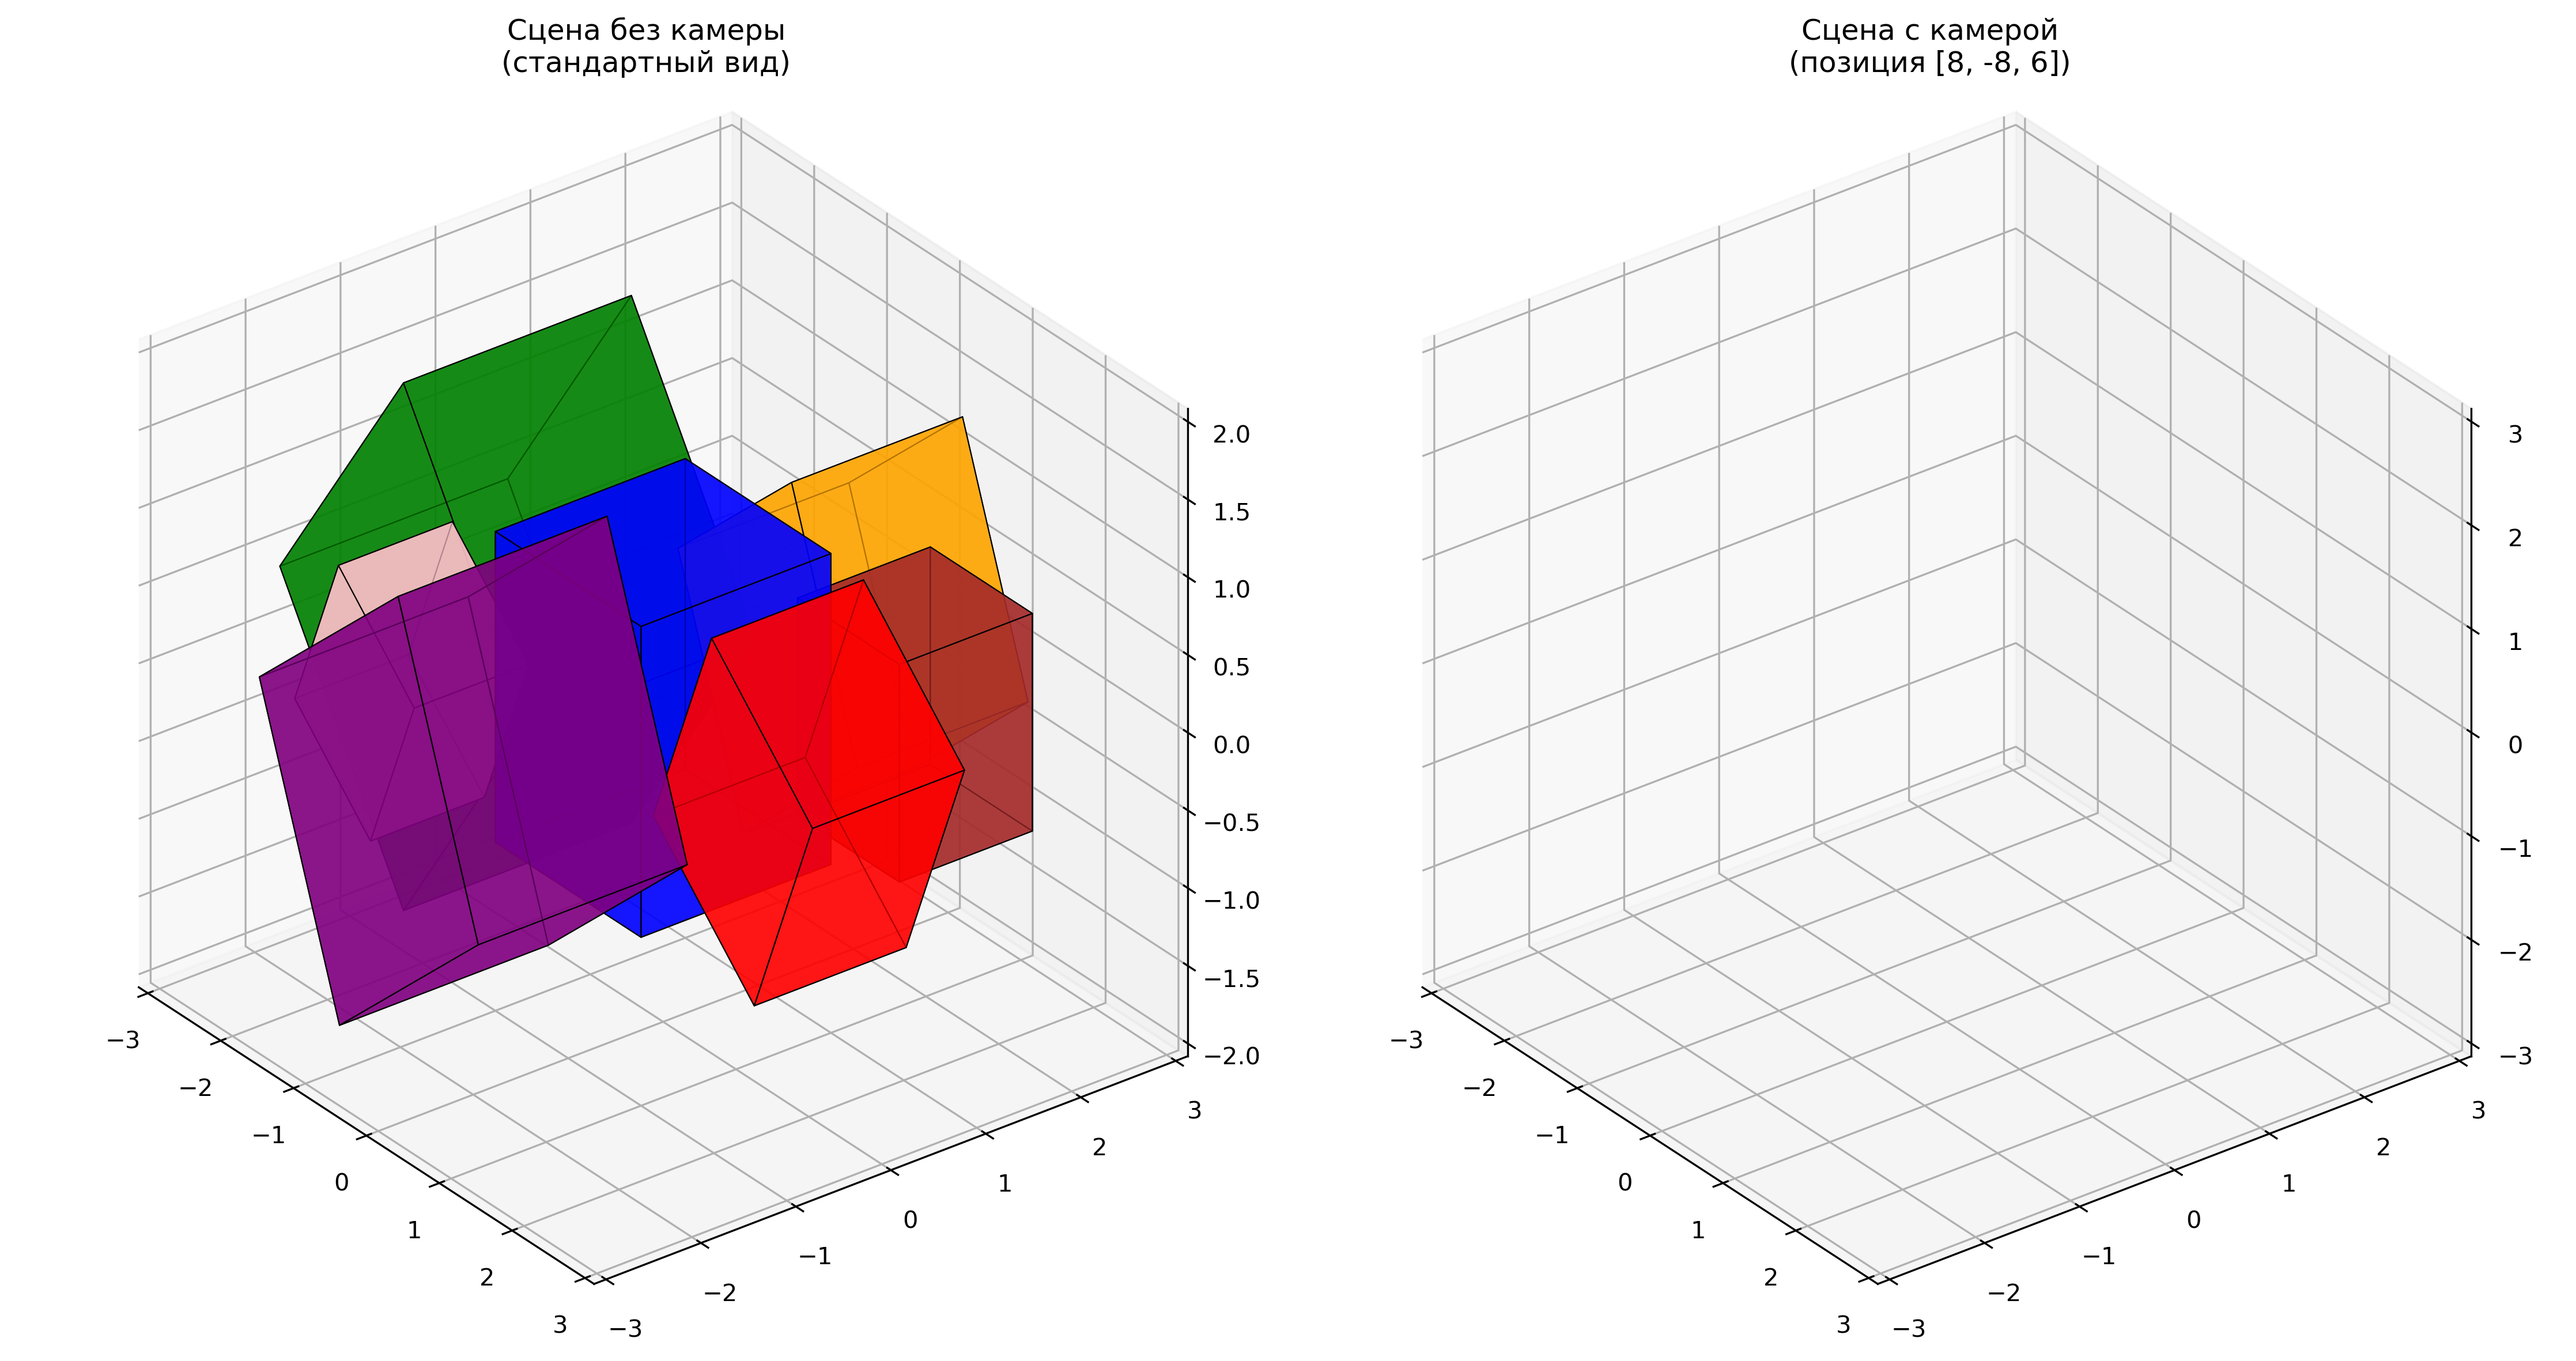
\includegraphics[width=\textwidth]{images/task6/camera_effect_comparison.png}
\caption{Сравнение сцены с камерой и без камеры}
\label{fig:camera_effect_comparison}
\end{figure}

\section*{Задание 7: Реализация перспективы}

\subsection*{Матрица перспективной проекции}

Матрица перспективной проекции $P$ имеет вид:

\begin{equation}
P = \begin{bmatrix}
\frac{f}{\text{aspect}} & 0 & 0 & 0 \\
0 & f & 0 & 0 \\
0 & 0 & \frac{\text{far} + \text{near}}{\text{near} - \text{far}} & \frac{2 \cdot \text{far} \cdot \text{near}}{\text{near} - \text{far}} \\
0 & 0 & -1 & 0
\end{bmatrix}
\end{equation}

где $f = \frac{1}{\tan(\text{FOV}/2)}$ - фокусное расстояние.

\subsection*{Параметры перспективы}

\begin{itemize}
\item \textbf{FOV (Field of View)}: угол поля зрения в градусах
\item \textbf{Aspect Ratio}: соотношение сторон экрана
\item \textbf{Near Plane}: ближняя плоскость отсечения
\item \textbf{Far Plane}: дальняя плоскость отсечения
\end{itemize}

\begin{figure}[h]
\centering
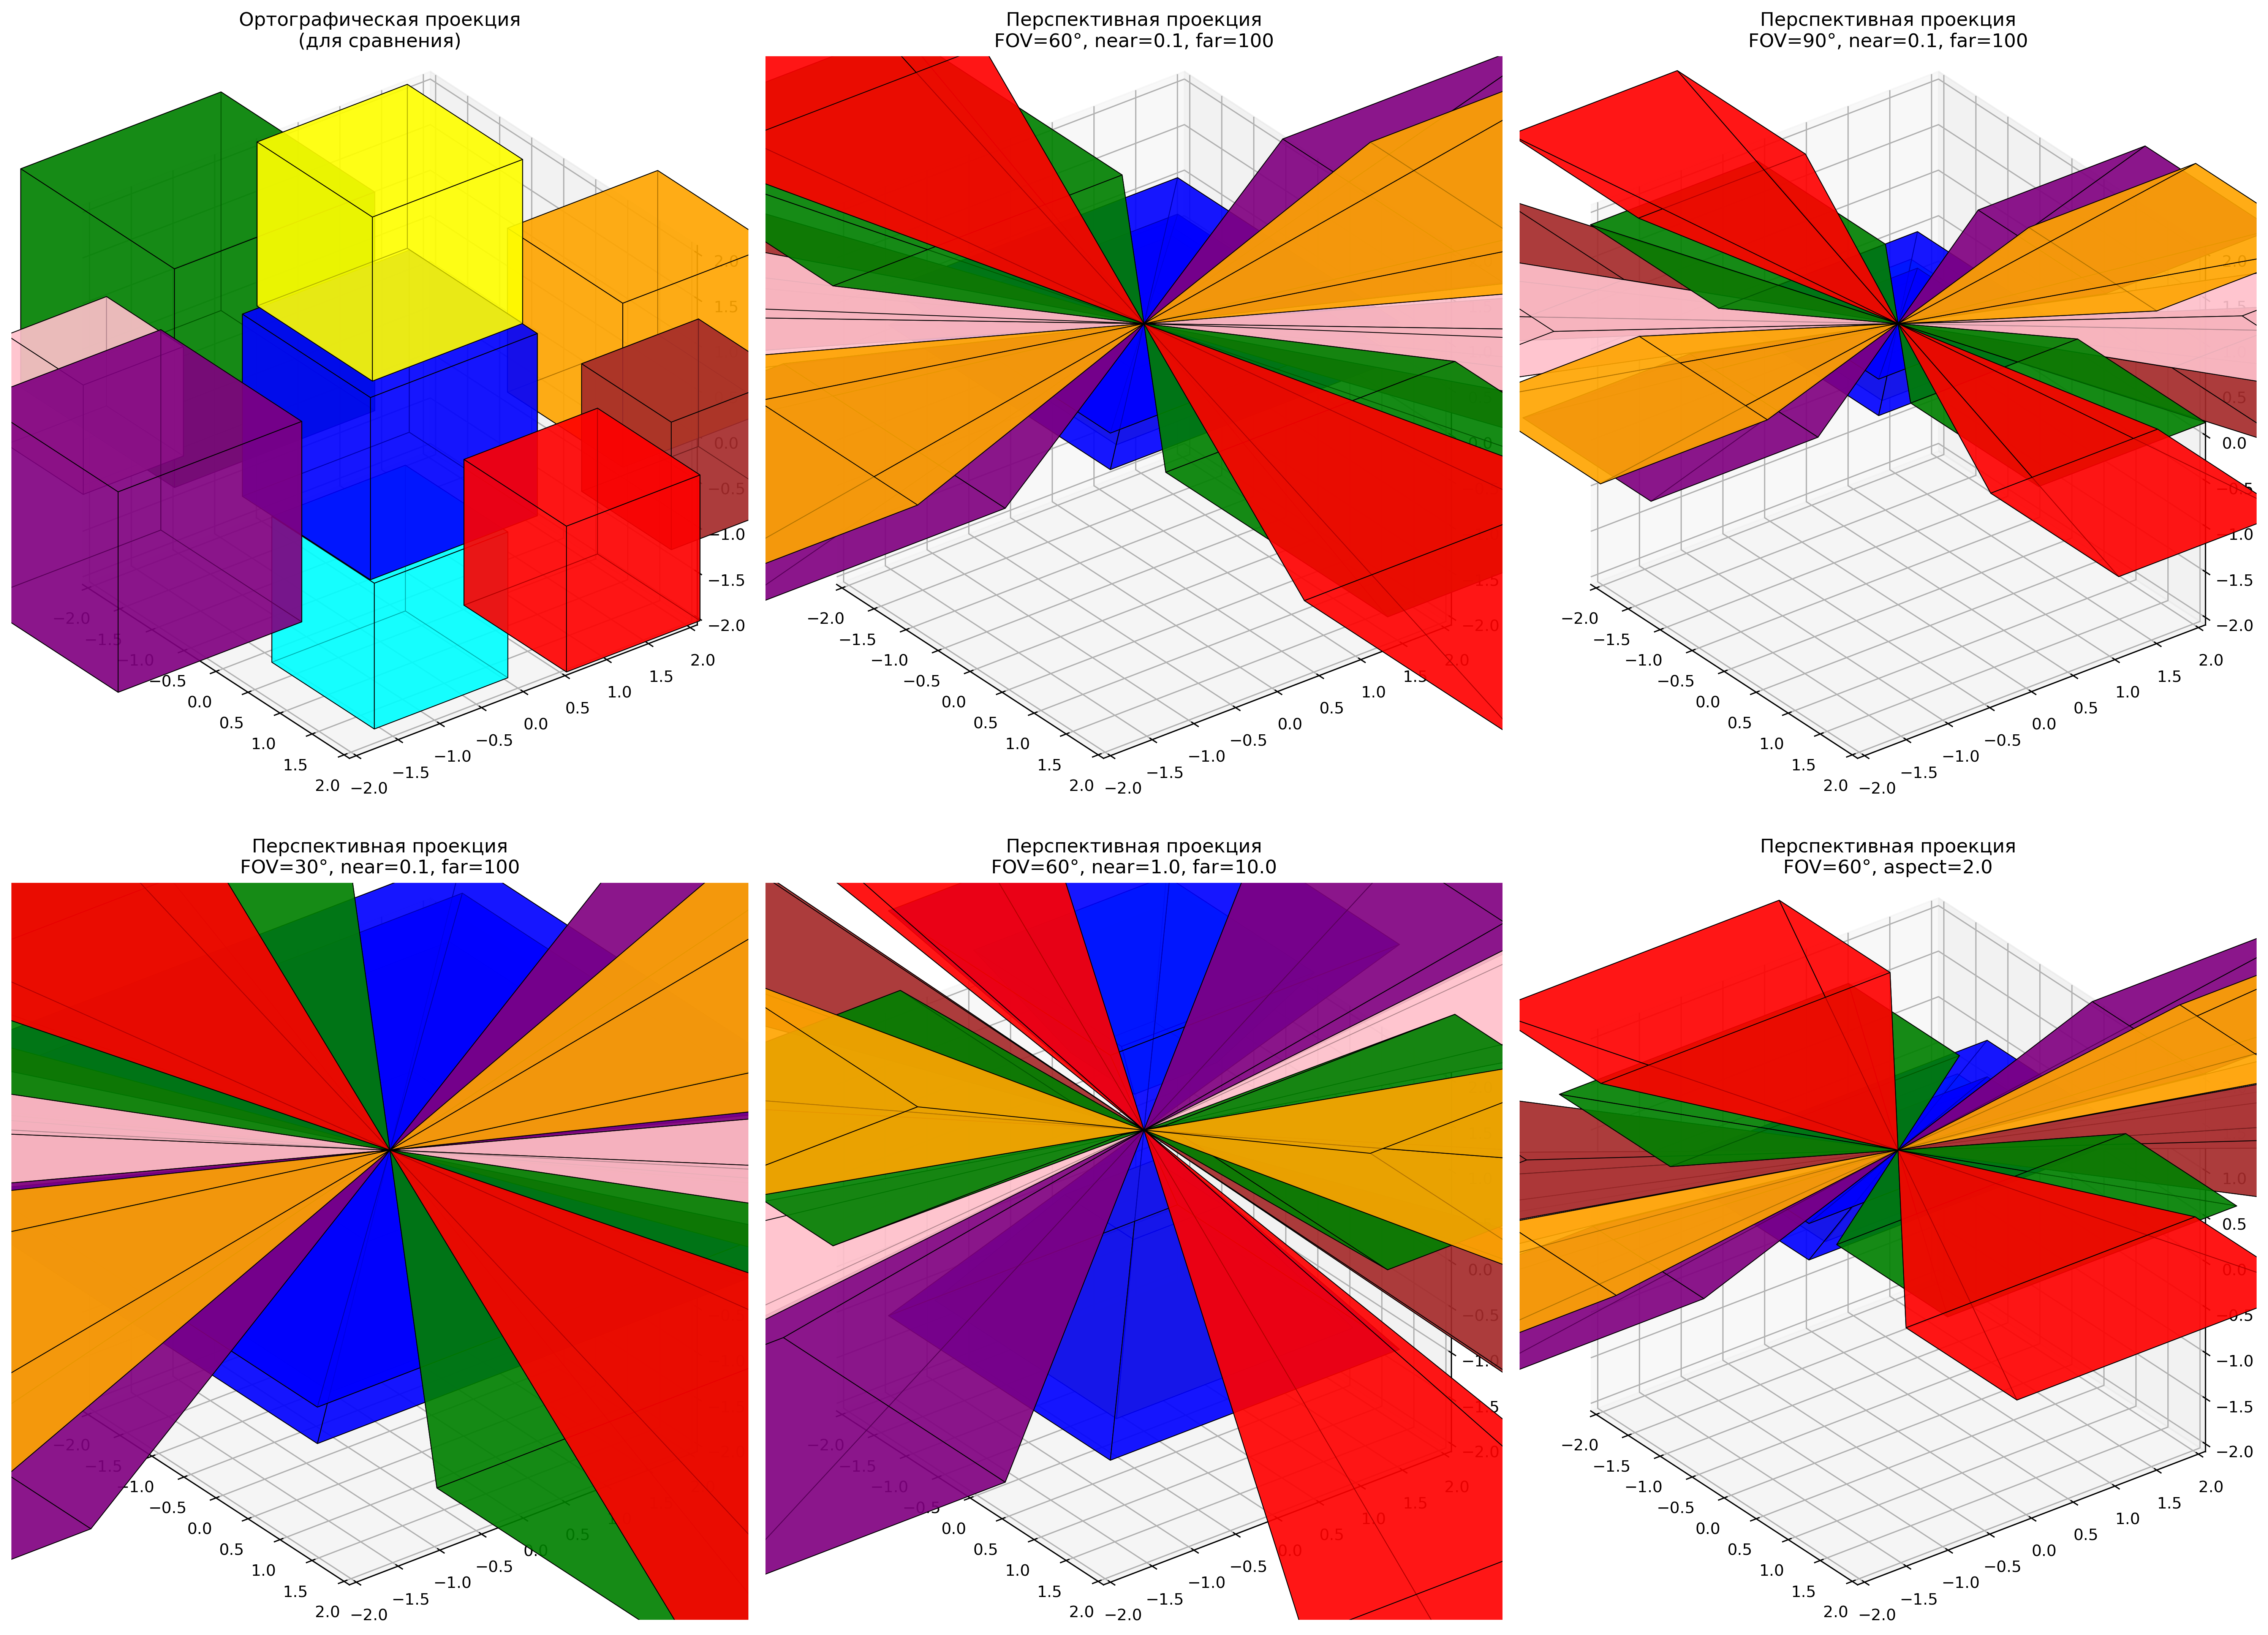
\includegraphics[width=\textwidth]{images/task7/perspective_projections.png}
\caption{Перспективные проекции с различными параметрами}
\label{fig:perspective_projections}
\end{figure}

\subsection*{Сравнение с ортографической проекцией}

\begin{figure}[h]
\centering
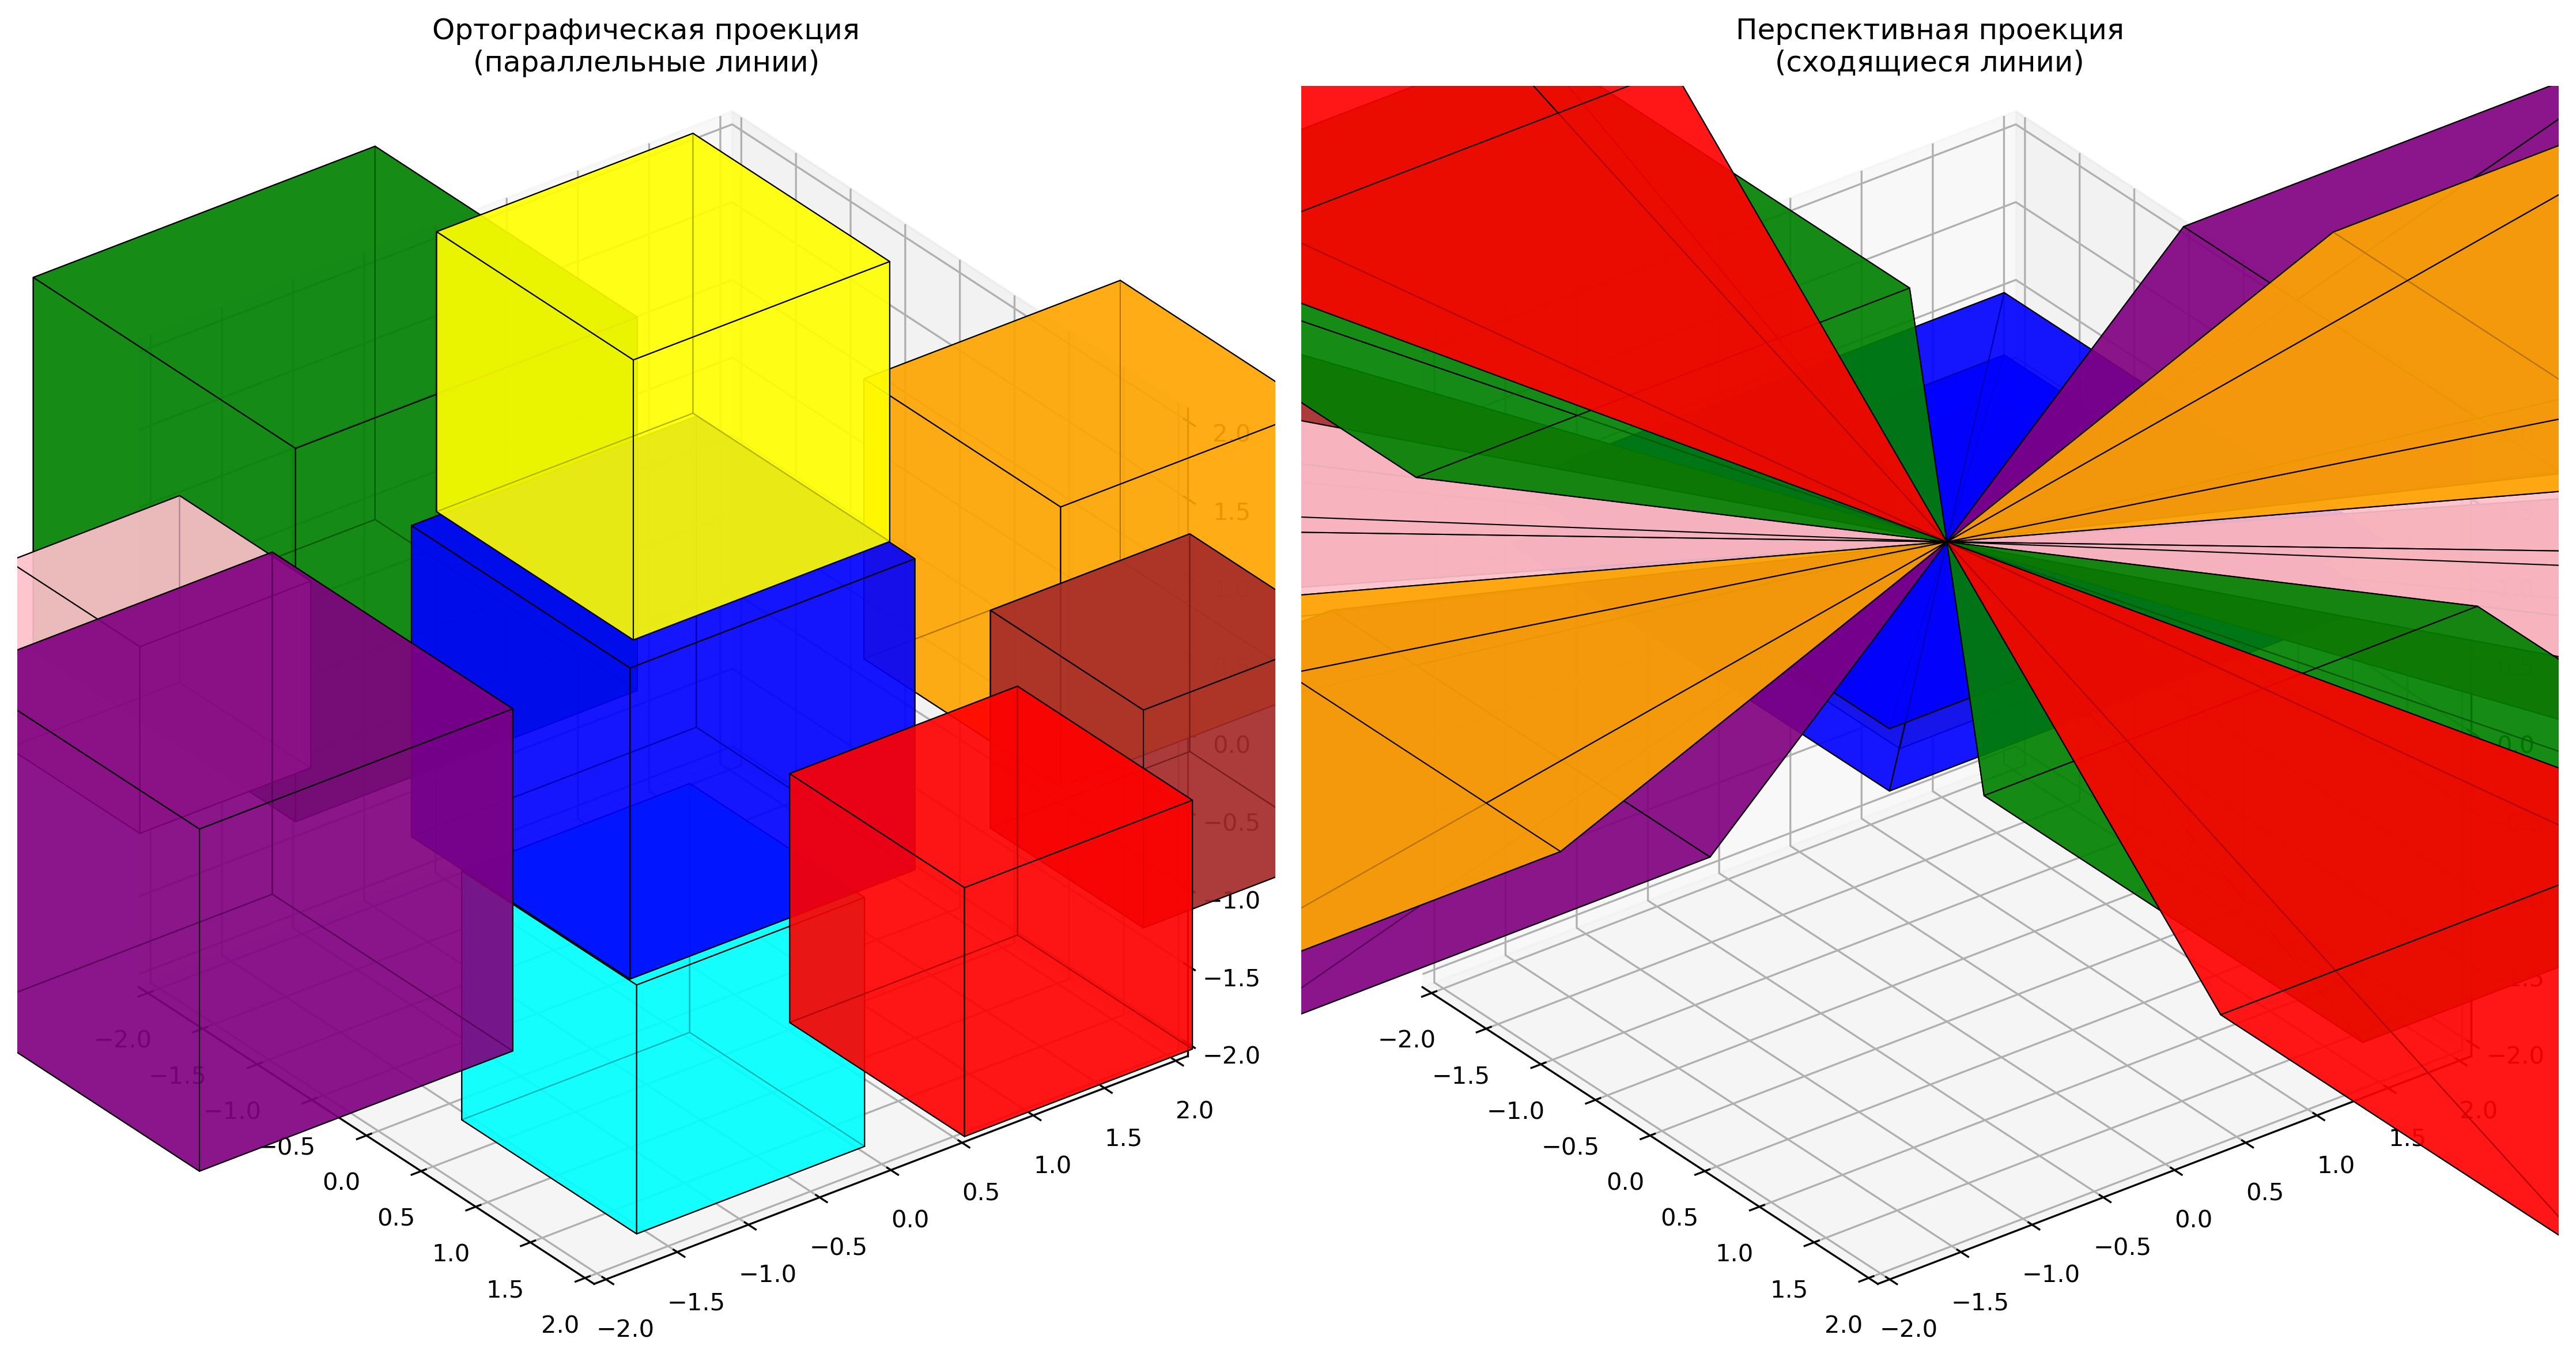
\includegraphics[width=\textwidth]{images/task7/orthographic_vs_perspective.png}
\caption{Сравнение ортографической и перспективной проекций}
\label{fig:orthographic_vs_perspective}
\end{figure}

\subsection*{Структура матрицы перспективы}

Матрица перспективы $P$ имеет следующую структуру:
\begin{itemize}
\item \textbf{Первые два элемента}: Масштабирование по осям X и Y в зависимости от FOV и aspect ratio
\item \textbf{Третий элемент}: Преобразование координаты Z для создания эффекта глубины
\item \textbf{Четвертый элемент}: Перенос в координату W для перспективного деления
\item \textbf{Последняя строка}: $[0, 0, -1, 0]$ - ключевой элемент для перспективного деления
\end{itemize}

\subsection*{Параметры матрицы}

\begin{itemize}
\item \textbf{FOV (Field of View)}: Определяет угол обзора камеры (обычно 45-90°)
\item \textbf{Aspect Ratio}: Соотношение ширины к высоте экрана
\item \textbf{Near Plane}: Ближняя плоскость отсечения (обычно 0.1-1.0)
\item \textbf{Far Plane}: Дальняя плоскость отсечения (обычно 100-1000)
\end{itemize}

\subsection*{Исследование деформации пространства}

Используется стандартное вращение графика для исследования того, как перспективная проекция деформирует пространство. Дальние объекты становятся меньше, создавая эффект глубины.

\subsection*{Эффект расстояния}

\begin{figure}[h]
\centering
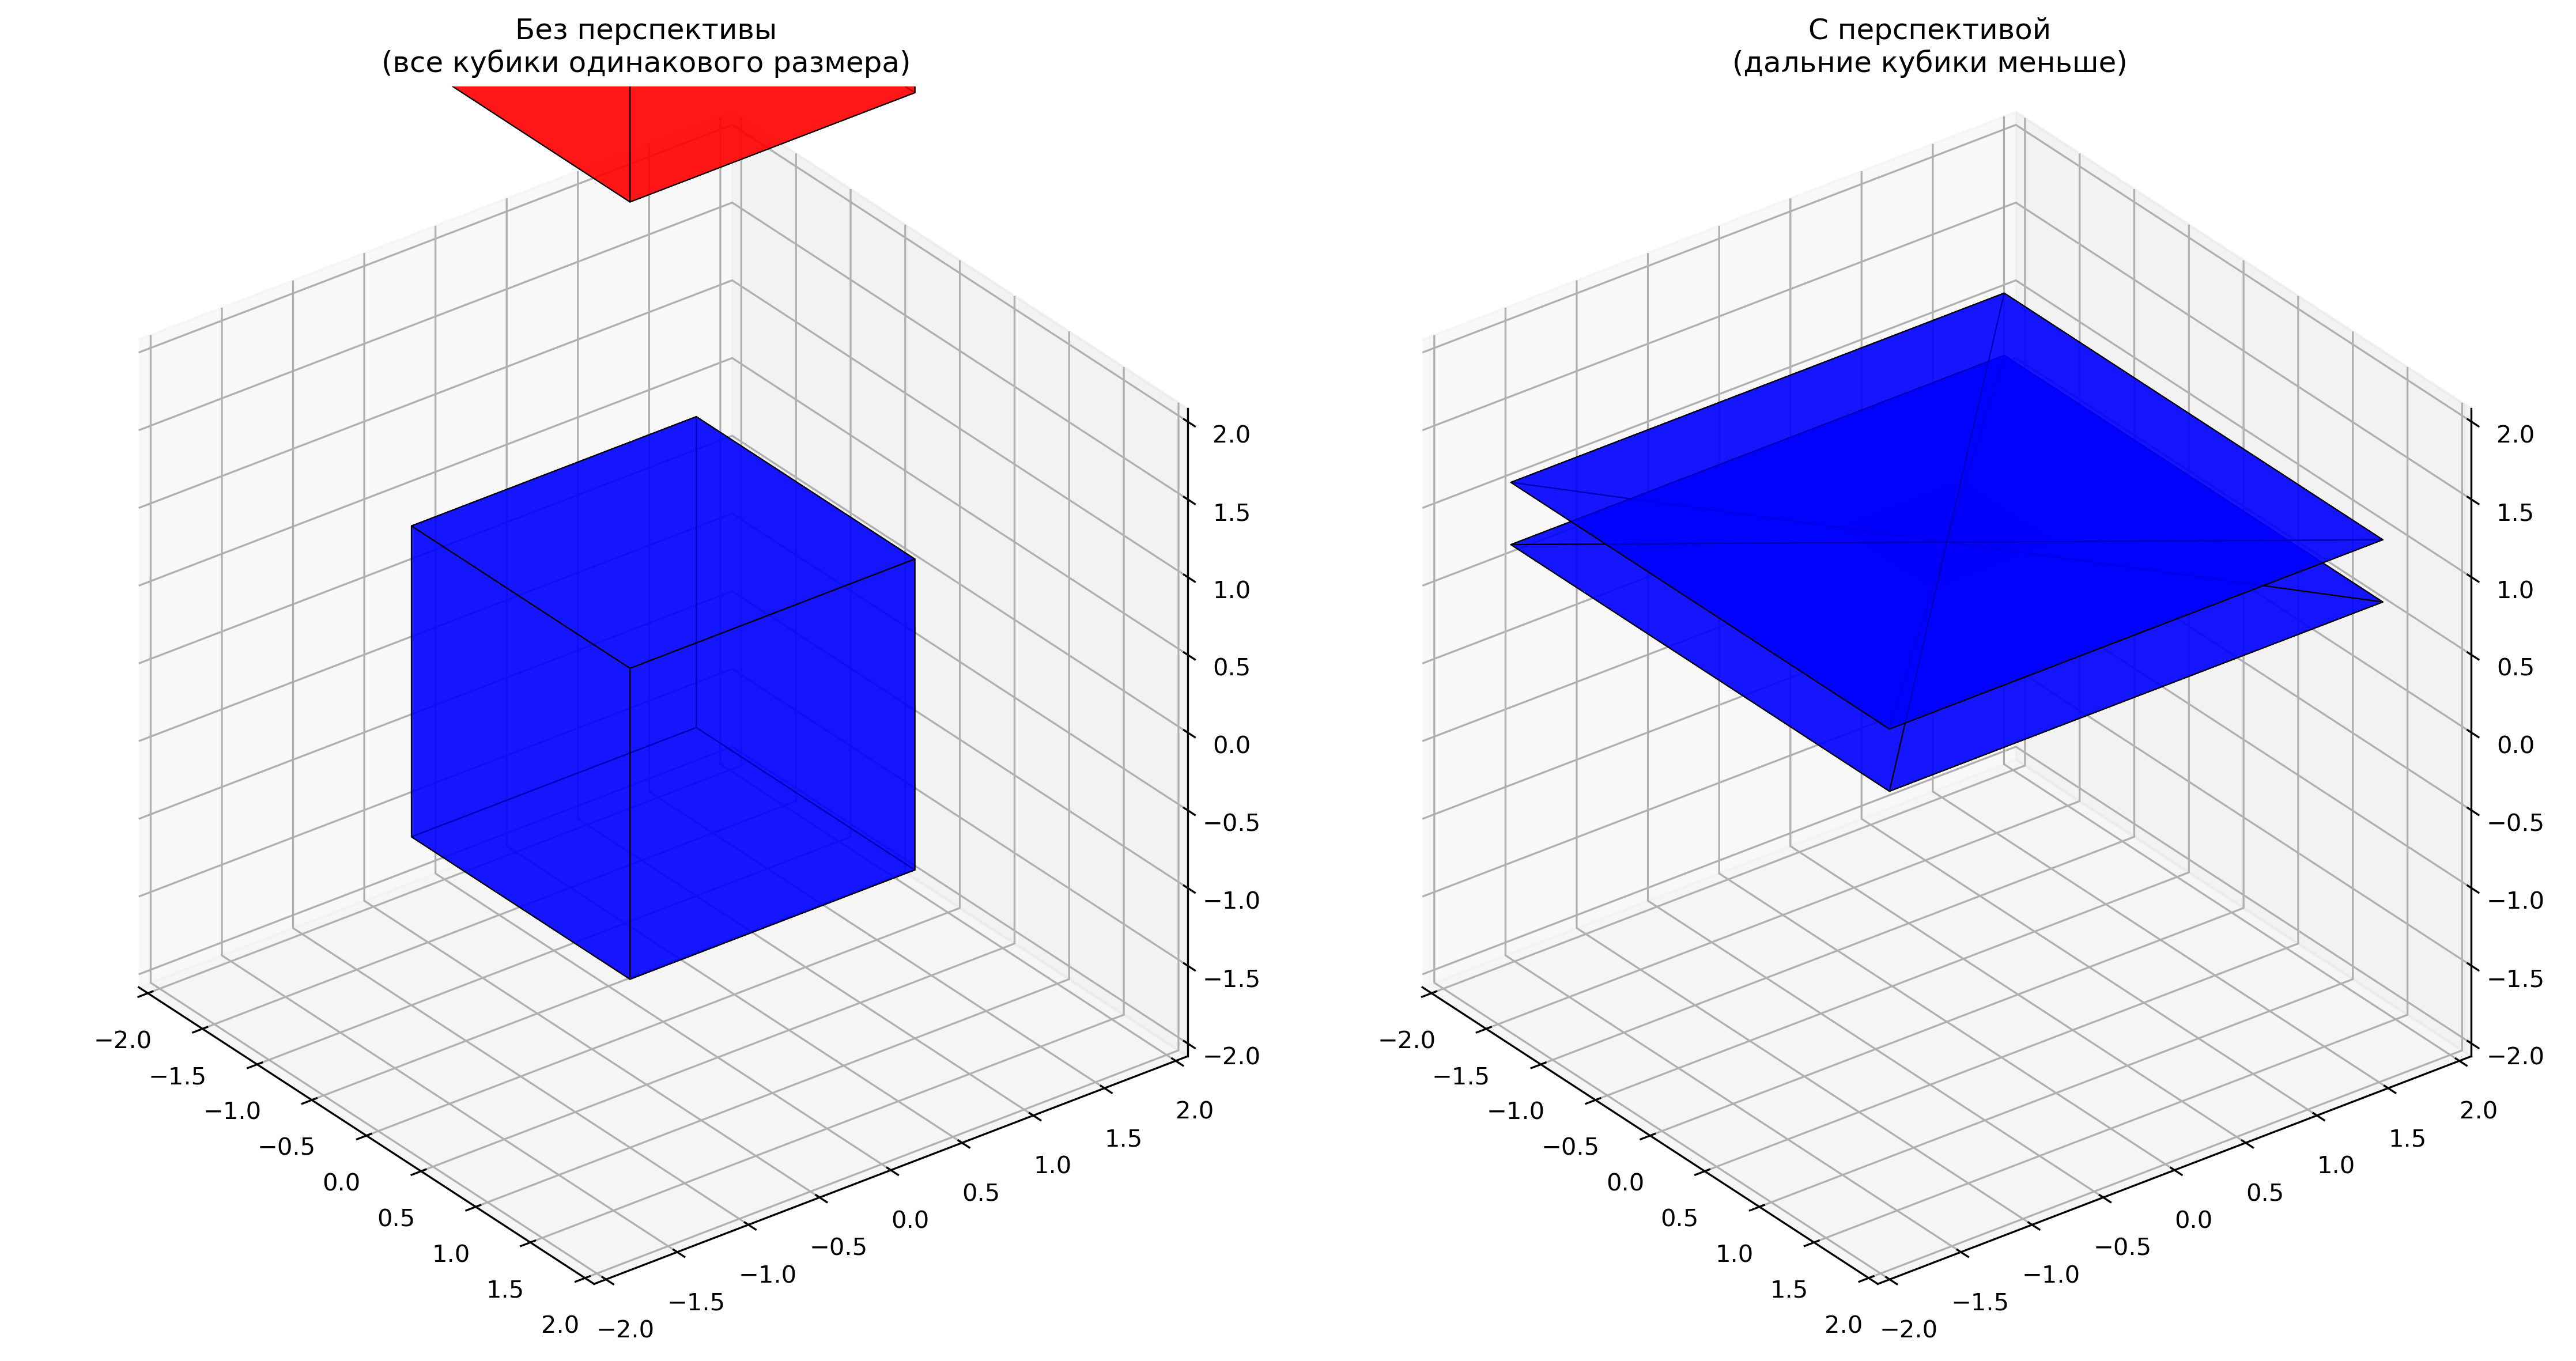
\includegraphics[width=\textwidth]{images/task7/distance_effect_perspective.png}
\caption{Эффект расстояния в перспективной проекции}
\label{fig:distance_effect_perspective}
\end{figure}

\section*{Основные результаты}

\subsection*{Ключевые выводы}

\begin{enumerate}
\item \textbf{Однородные координаты} позволяют объединить линейные и аффинные преобразования в единую матричную форму.

\item \textbf{Некоммутативность преобразований}: порядок применения матриц важен. $TS \neq ST$, $TR \neq RT$.

\item \textbf{Вращение вокруг произвольной оси} можно реализовать с помощью экспоненциальной матрицы $R_{\mathbf{v}}(\theta) = e^{J\theta}$.

\item \textbf{Теорема вращения Эйлера} утверждает, что любое вращение можно представить как композицию трех вращений вокруг координатных осей.

\item \textbf{Матрица камеры} позволяет преобразовать сцену так, как будто камера находится в начале координат.

\item \textbf{Перспективная проекция} создает эффект глубины, делая дальние объекты меньше ближних.

\end{enumerate}

\subsection*{Практическая значимость}

Полученные результаты имеют важное значение для:

\begin{itemize}
\item Разработки 3D-графических приложений
\item Создания компьютерных игр
\item Моделирования в CAD-системах
\item Компьютерной анимации
\item Визуализации научных данных
\end{itemize}

\subsection*{Математические основы}

Все преобразования в данной работе основаны на матричной алгебре и теории групп преобразований. Использование однородных координат позволяет представить все аффинные преобразования в виде матричного умножения, что обеспечивает эффективную реализацию в компьютерной графике.

\section*{Заключение}

В ходе выполнения лабораторной работы №3 были успешно изучены и реализованы основные матричные преобразования, используемые в 3D-графике:

\begin{itemize}
\item Создание и отрисовка базовых 3D объектов
\item Масштабирование и перемещение объектов
\item Вращение вокруг произвольных осей
\item Реализация системы камеры
\item Перспективная проекция
\end{itemize}

Все преобразования были реализованы с использованием матриц $4 \times 4$ в однородных координатах, что обеспечивает единообразный подход к различным типам преобразований. Полученные результаты демонстрируют фундаментальные принципы компьютерной графики и могут быть использованы для дальнейшего изучения более сложных алгоритмов 3D-рендеринга.
